\documentclass[12pt, block=fill]{beamer}
\usepackage{graphicx}
\usepackage[sfdefault]{FiraSans}
\usepackage{FiraMono}
\usepackage[T1]{fontenc}
\usepackage{xcolor}
\usepackage{mathtools}

\usepackage{hyperref}
\usepackage{tabularx}

\definecolor{burntOrange}{rgb}{.8, .5, .1}
\definecolor{textgray}{rgb}{.8,.8,.8}
\definecolor{berkeleyYellow}{HTML}{FDB515}

\newcommand{\alex}[1]{\textcolor{berkeleyYellow}{#1}}
\newcommand{\paul}[1]{\textcolor{red}{#1}}




\usetheme[
titleformat frame = smallcaps,
subsectionpage = progressbar]
{metropolis}

\metroset{
  block=fill
}

\newcommand{\E}{\text{E}}
\newcommand{\V}{\text{V}}

\newcommand{\Z}{\mathbb{Z}}
\newcommand{\R}{\mathbb{R}}
\newcommand{\N}{\mathbb{N}}
\newcommand{\indep}{\mathrel{\text{\scalebox{1.07}{$\perp\mkern-10mu\perp$}}}}

\usepackage{pgfpages}
\setbeameroption{hide notes} % Only slides
% \setbeameroption{show only notes} % Only notes
%   \setbeameroption{show notes on second screen=right} % Both


 \title{Week 2}
 \subtitle{Introduction to Probability}

 \author{Paul Laskowski and Alex Hughes}
 \institute{UC Berkeley, School of Information}

\begin{document}

\begin{frame}
\maketitle
\end{frame} 

\begin{frame} 
\footnotesize
\tableofcontents[hideallsubsections]
\end{frame}

\section{Introduction}
\subsection{Motivating Examples}

\begin{frame}
  \frametitle{Plan for the Week}
  Two sections:
  \begin{enumerate}
  \item Defining random variables
  \item Joint distributions
  \end{enumerate}

  \note[item]{This is a foundation week.}  \note[item]{Random
    Variables are building blocks of statistical models.}
  \note[item]{Thinking of the analogy with Jazz music, you'll want
    your understanding of them to be rock solid.}  \note[item]{So
    we're going to be very mathematically precise in defining what
    these are.}  \note[item]{We'll have three sections...}
\end{frame}

\begin{frame}
  \frametitle{Plan for the Week (cont.)}
  At the end of this week, you will be able to:
  \begin{itemize}
  \item Understand how random variables fit as a part of statistical
    modeling
  \item Apply the mathematical tools we have for characterizing random
    variables
  \item Solve problems by applying properties of expectation and
    variance
  \end{itemize}
  \note[item]{}
\end{frame}

\section{Part 1: Introducing Random Variables}
% \section{Introducing Random Variables}

\subsection{Introduction Random Variables}
\begin{frame}
  \frametitle{What Is a Random Variable?}
  Intuition:
  \begin{itemize}
  \item A model for where the numbers in data come from.
  \item Like a regular variable but with uncertainty about its value. \note[item]{with
    some probability of taking on different values}

  \end{itemize}
  
  \begin{block}{Random Variable}
  Given probability space $(\Omega, S, P)$, a \textit{random variable} is a measurable function from $\Omega$ to  $\mathbb{R}$.
  \end{block}
  \note[item]{A Random Variable is the fundamental building block of a
    statistical model, but what is it?}  \note[item]{Intuitively,
    we're used to variables in our datasets.  They have one value.
    But as statisticians we need a way to model variables
    acknowledging that different values are possible}
  \note[item]{Finally, we have the formal definition that you'll see
    in your textbook.  A random variable is a function from a
    probability space to R.  This one, unfortunately, leaves students
    scratching their heads.  It doesn't seem to capture the
    intuition.}
\end{frame}


\begin{frame}[t]
  \frametitle{What Is a Random Variable (Formally)?}
  \centering
  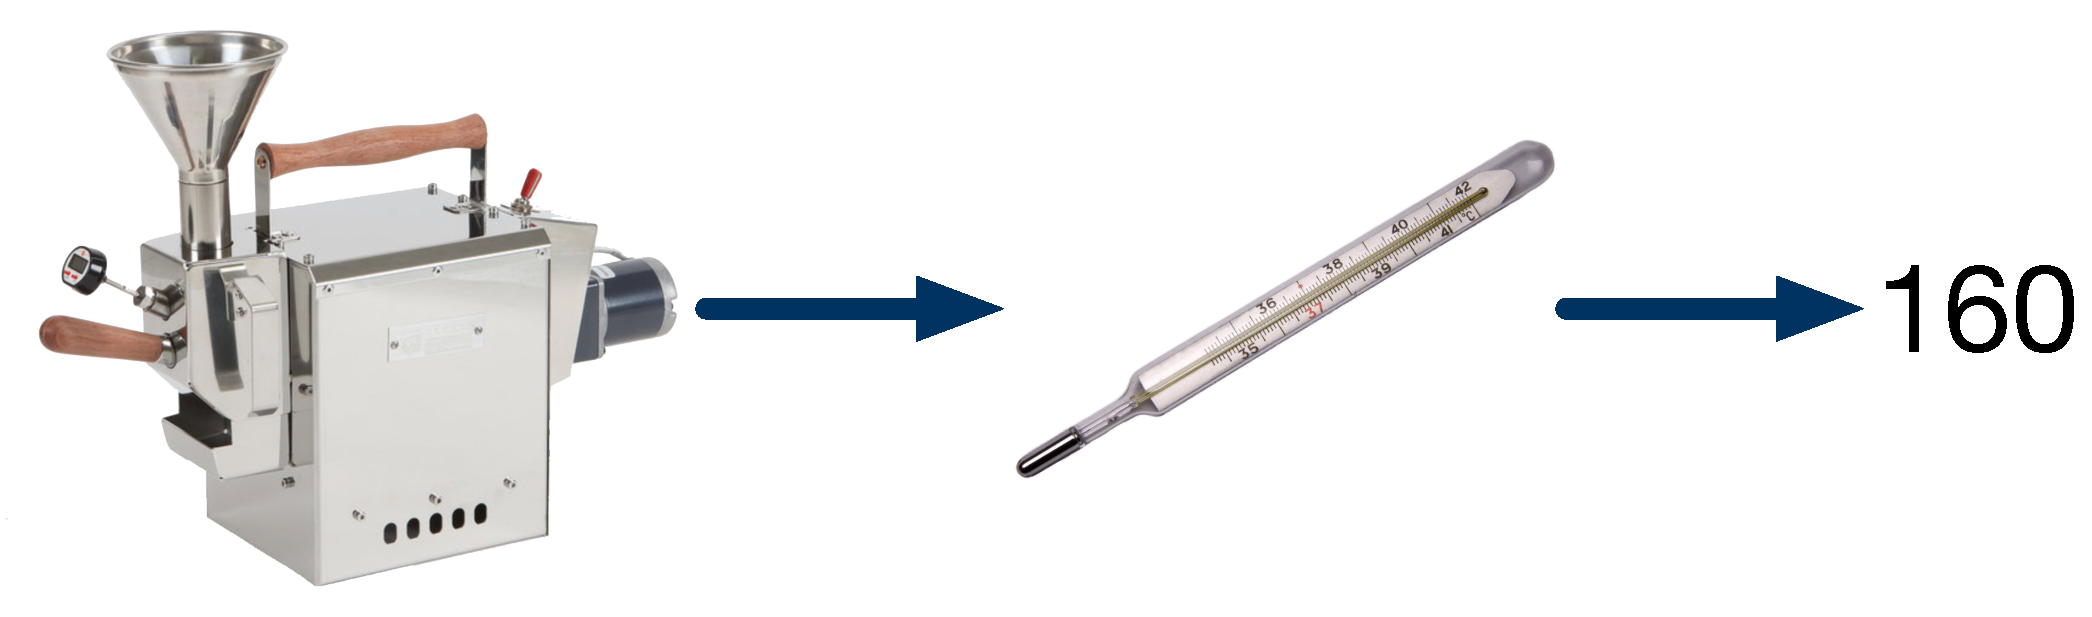
\includegraphics[width= \textwidth ]{figures/roaster1}
  \note[item]{I'm going to try to make the formal definition make more
    sense.  And I'll do it by telling a very stylized story about how
    a variable gets the value it has.}  \note[item]{This story is
    about something I do in my spare time, which is roast coffee.  It
    has three characters.}  \note[item]{The first character is my
    coffee roaster.  This is in the actual real world.  It has some
    state: the atoms are moving with some velocity, the proteins in
    the beans are in some configuration - hopefully the proteins
    aren't burnt.}  \note[item]{Because I'm serious about my roasting,
    I want some data.  So the second character is this thermometer.
    It represents measurement or observation.  Think of the state of
    the roaster as an input to the thermometer} \note[item]{The final
    character is the output of the thermometer: a regular old
    variable.  160 degrees.}
\end{frame}

\begin{frame}[t]
  \frametitle{What Is a Random Variable (Formally)?}
  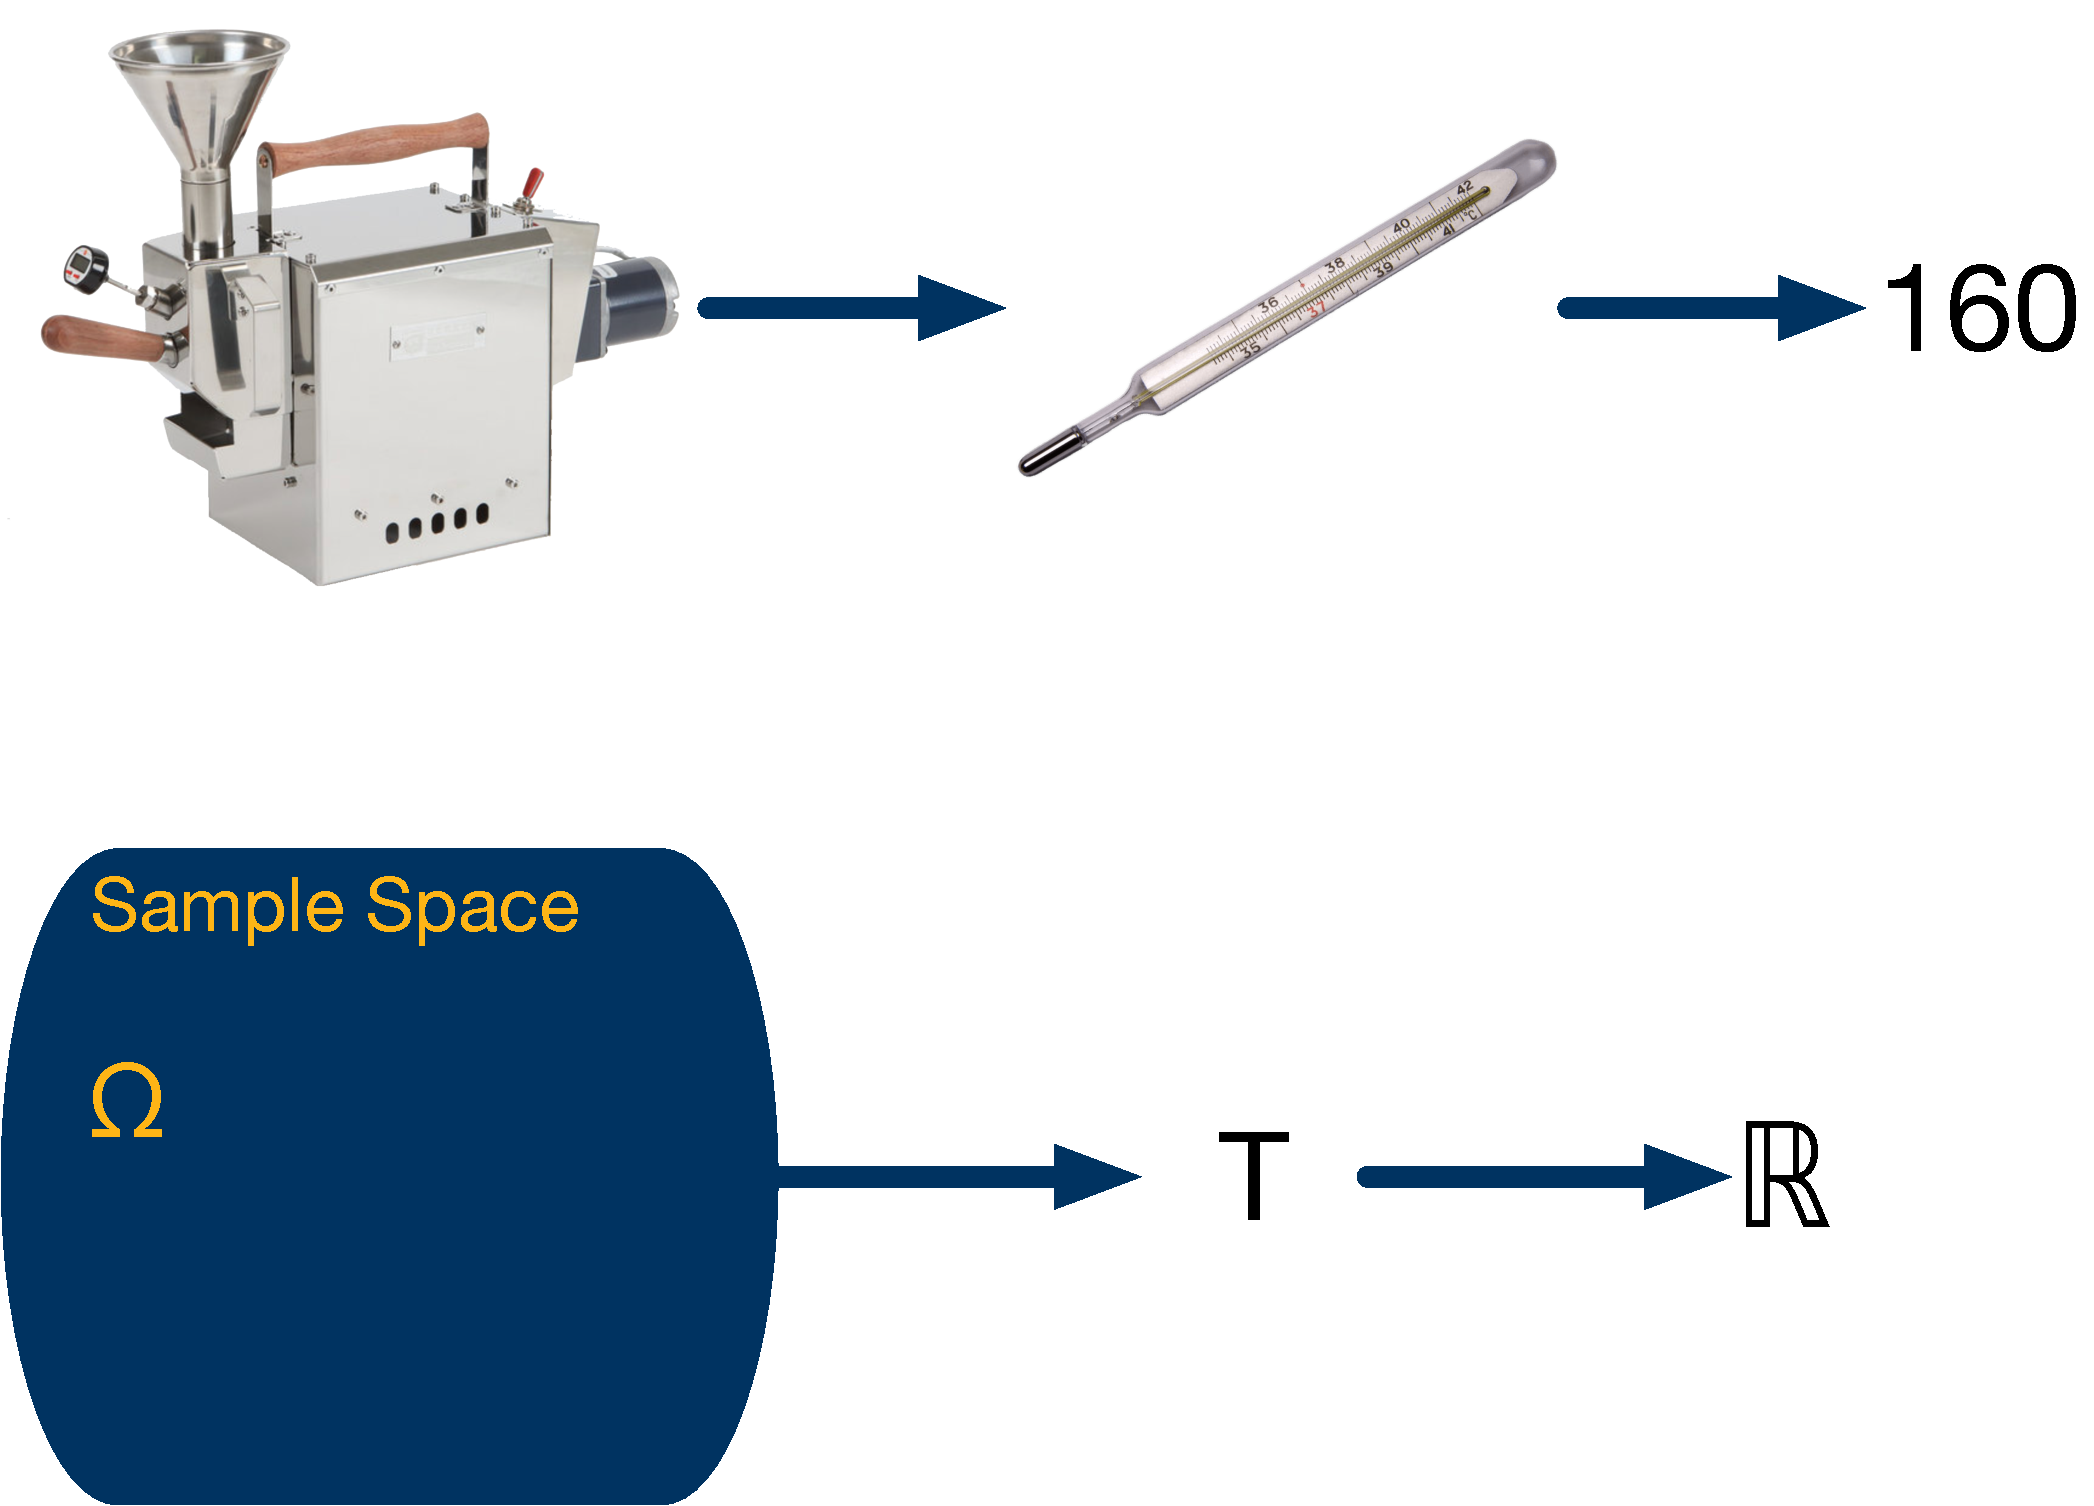
\includegraphics[width= \textwidth ]{figures/roaster2}

  \note[item]{Now as statisticians, we think that there must be some
    randomness in that number.  In other words, if you could magically
    rewind time and start roasting again, you might get a different
    number.  You might not actually believe this - if we could
    recreate the start of the experiment EXACTLY, down to the location
    of atoms, maybe you think you'd get the same number.  But at least
    as statisticians, we want a model for how this number was created
    that involves randomness.  Here's how we do it...}
  \note[item]{First, we need a probability space.  Each outcome in
    this space represents one possible state of my coffee roaster.
    There is a probability function that tells you how probable
    different states are.}
      \note[item]{Next, we have the random variable.  this is like the
    thermometer, but it doesn't give us a single number.  it's a
    function that takes in any outcome - any state of the coffee
    roaster.}
    \note[item]{Finally, the last character is the real numbers.  The
    random variable is a function from omega to the reals.}
\end{frame}

\begin{frame}[t]
  \frametitle{What Is a Random Variable (Formally)?}
  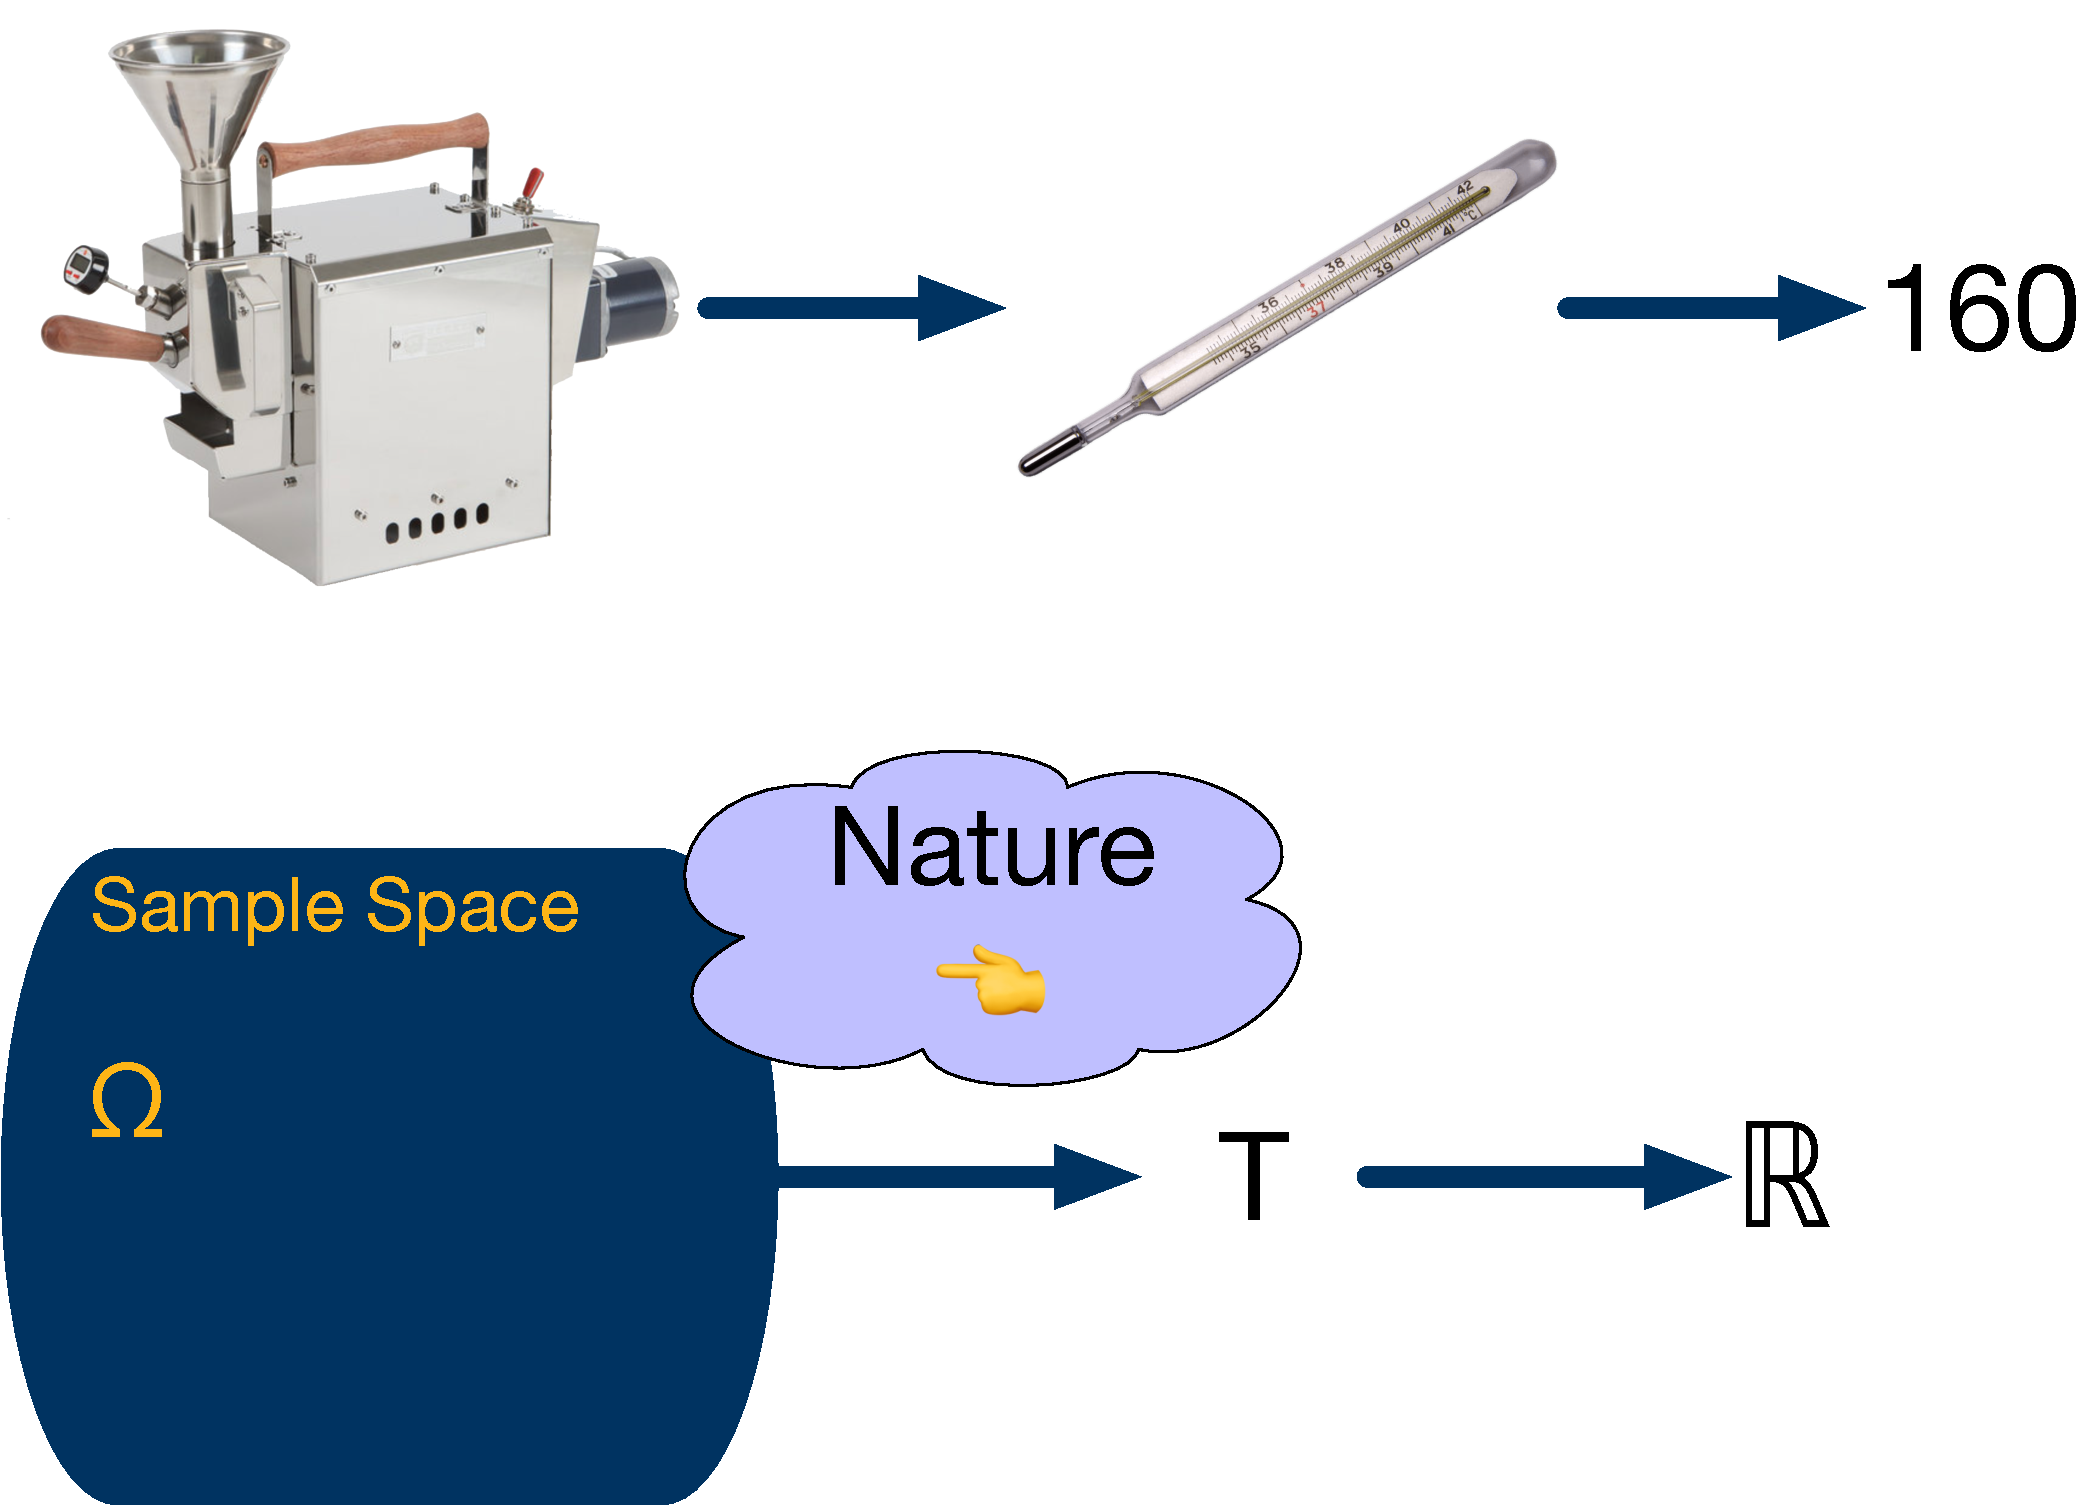
\includegraphics[width= \textwidth ]{figures/roaster3}
  \note[item]{That's the setup.  Let's see what happens when the
    experiment runs.}  \note[item]{First nature reaches in and selects
    one possible outcome.  remember this represents one possible
    arrangement of all the atoms in my roaster.}  \note[item]{Use
    Annotation, label outcome w, draw arrow to T, draw another arrow
    to 160.}
\end{frame}

\begin{frame}[t]
  \frametitle{Probabilities of Real Numbers}
  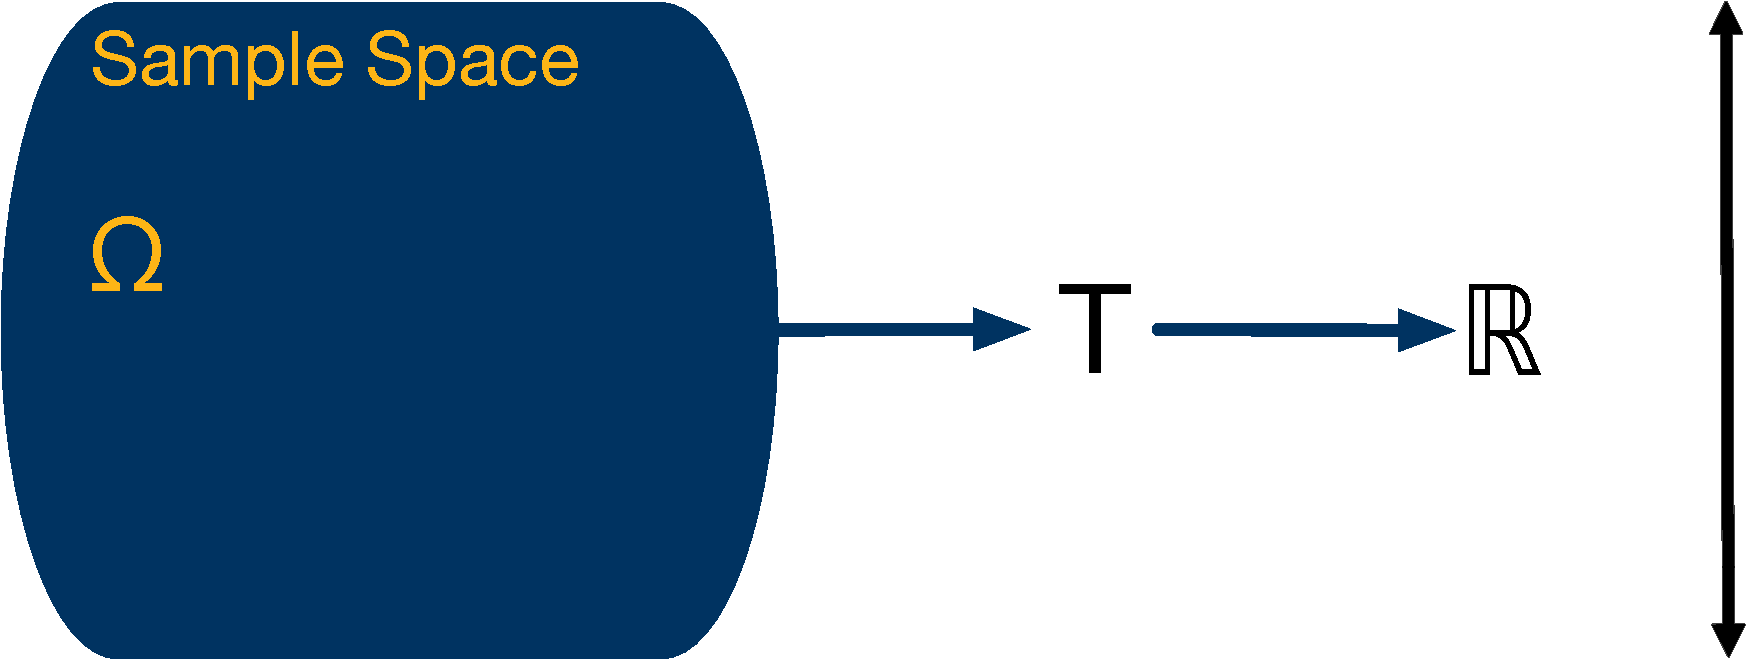
\includegraphics[width= \textwidth ]{figures/prob_space}
  \note[item]{Let me give you one more way to think about random
    variables.}  \note[item]{Here is our outcome space and the real
    number line.  The RV maps each outcome to a real number.}
  \note[item]{Remember that we have a probability measure on Omega.
    It turns out that the RV creates a new probability measure on R.
    Here's how: For any Set S of real numbers...}  \note[item]{If you
    know measure theory, you know that I wasn't 100\% correct.
    Technically, I need to assume that S is measurable.  Usually,
    we'll assume that S is in the Lesbegue sigma algebra.  Then the assumption that T is
    a measurable function guarantees that T inverse of S is
    measurable.  If you don't know measure theory, then these details
    are not something to worry about.  Just remember that the RV
    translates probabilities of outcomes to probabilities of real
    numbers.  Most of the time, it's actually this P' that we're going
    to work with directly, but sometimes it's helpful to go back and
    think about the original outcome space.}
\end{frame}

\subsection{Reading: Random Variables}
 
\begin{frame}
  \frametitle{Reading Assignment}
  Read \textit{Foundations of Agnostic Statistics}, section 1.2.0–1.2.1.
\end{frame}

\subsection{Functions, Events, and Operators}

\begin{frame}[t]
  \frametitle{Functions of a Random Variable}
  \centering
  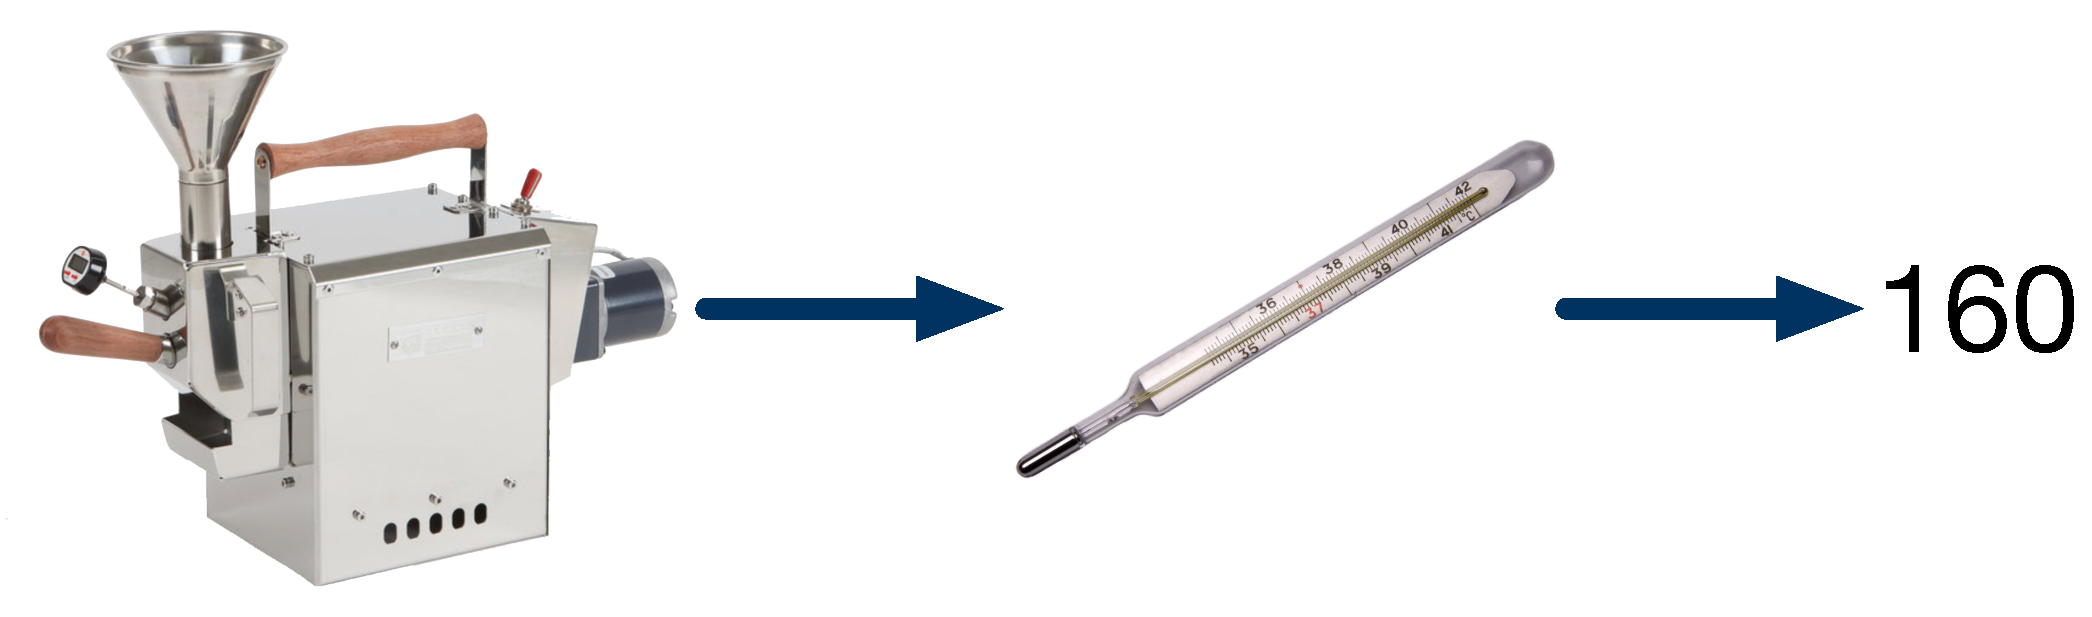
\includegraphics[width= .7 \textwidth ]{figures/roaster1}
  \begin{itemize}
  \item Random variable $T$ represents temperature in Fahrenheit, but
    you need Celsius.
  \end{itemize}
  \note[item]{Random variables are building blocks.  we don't just create them, we analyze them, which means we put them into equations and apply operations to them.  We create new random variables, and we create other types of mathematical objects.}
  \note[item]{Let's go over three basic examples, and we'll develop some vocabulary that will help us stay organized in the future.   }
  \note[item]{We have the temperature in Fahrenheit, but need celsius}
\note[item]{$f(t) = \frac{5}{9}(t-32)$}
\note[item]{We take the random variable T and put it into f, $f(T)$.  what kind of object is this?}
\end{frame}
  
\begin{frame}[t]
  \frametitle{Creating Events from a Random Variable}
  \centering
  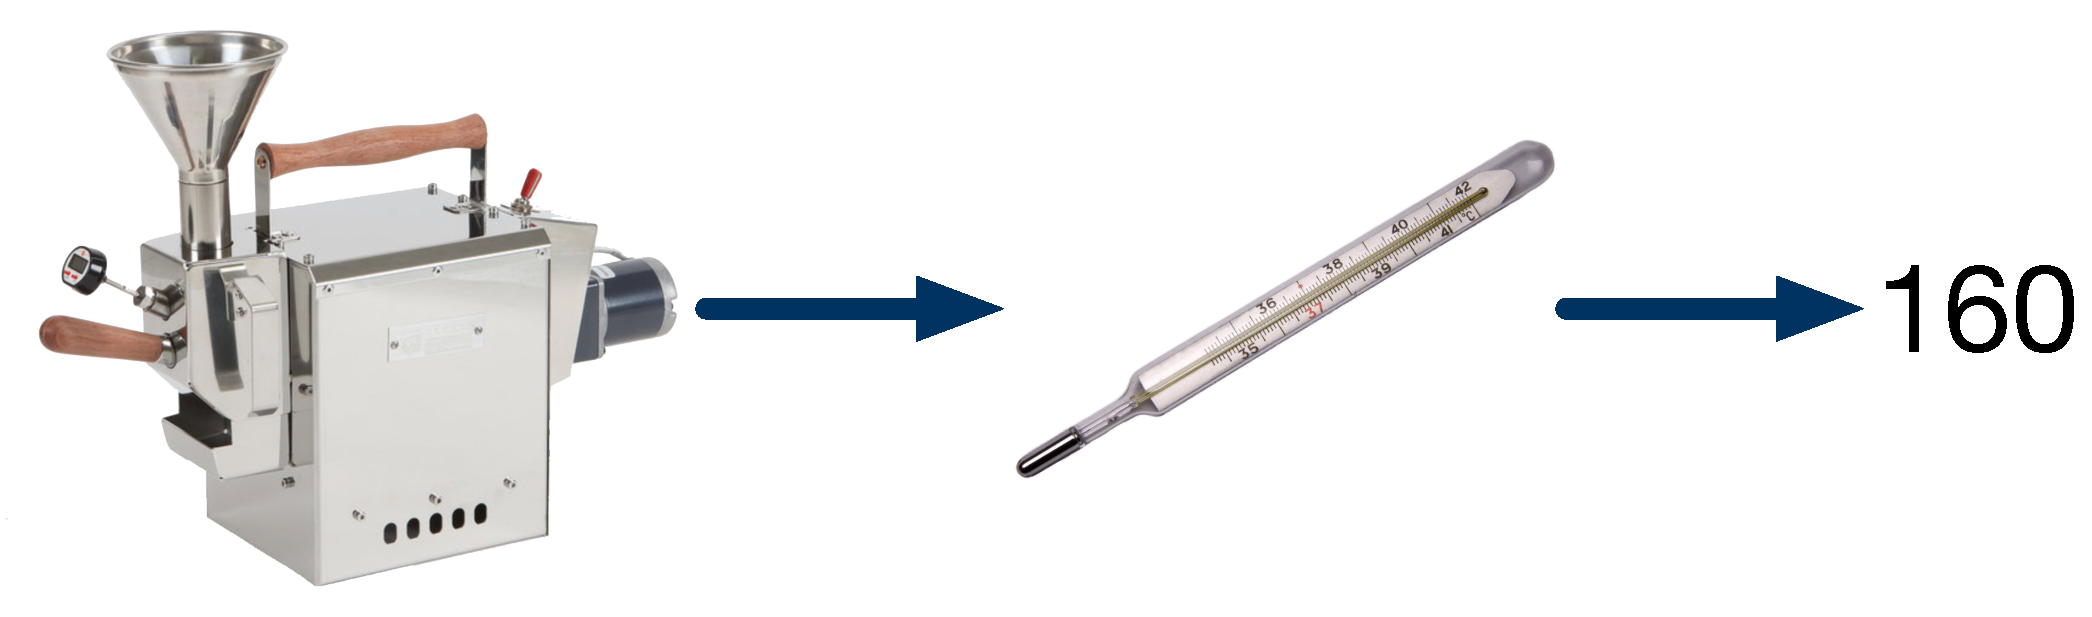
\includegraphics[width= .7 \textwidth ]{figures/roaster1}
    
  You want to know whether the temperature is below 150.
  \note[item]{You want to know if the temperature is below 150.  you
    write down T < 150.  what kind of thing is this?  It's an event!
    Let's draw the picture...}
\end{frame}

\begin{frame}[t]
  \frametitle{Operators Applied to a Random Variable}
  \centering
  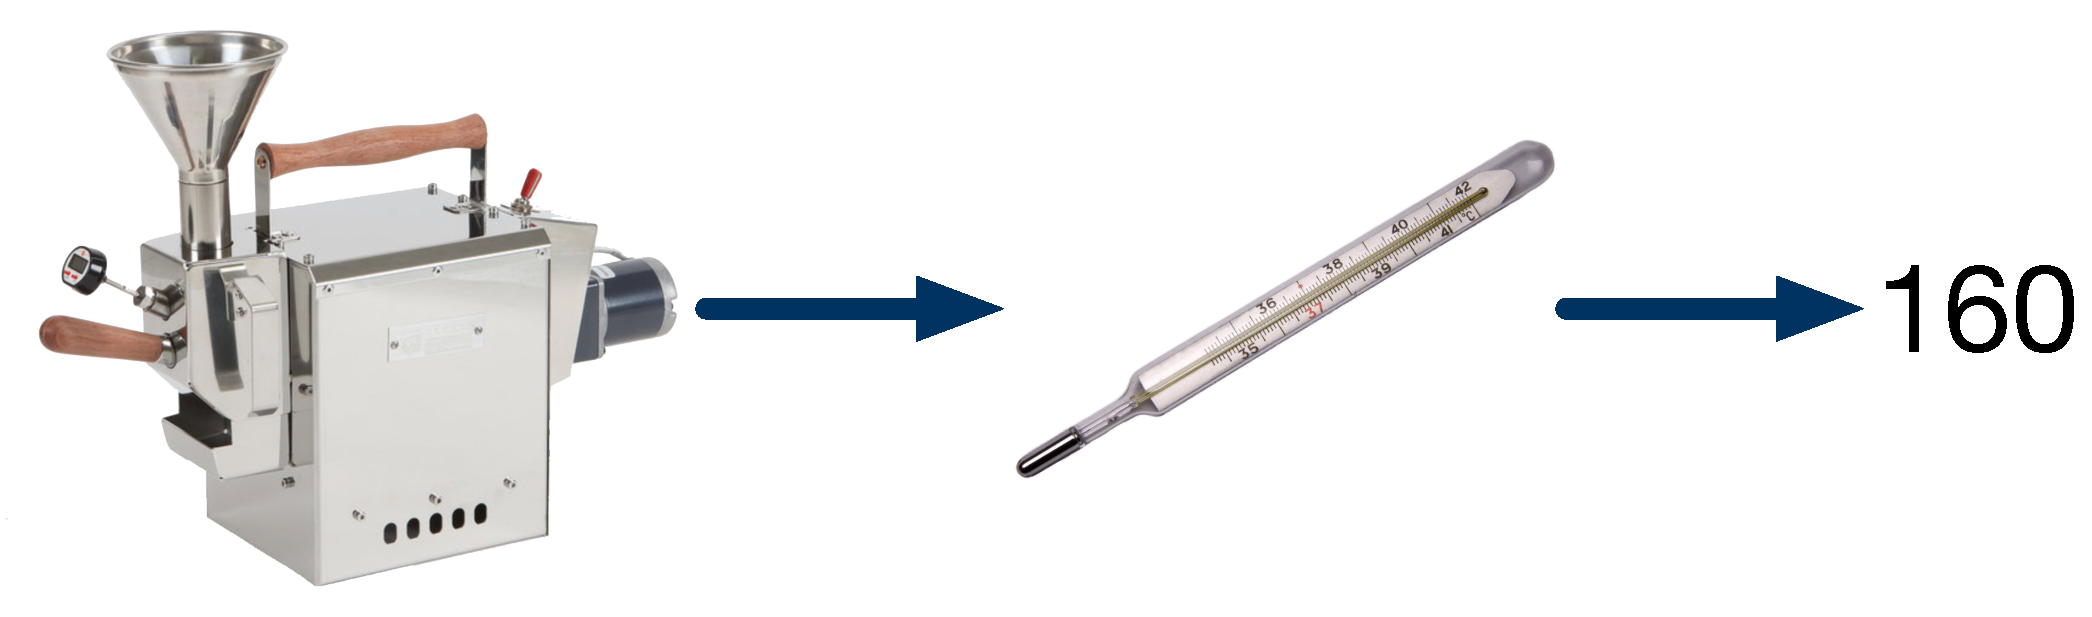
\includegraphics[width= .7 \textwidth ]{figures/roaster1}
  
  You want to know the minimum possible temperature.  \note[item]{you
    write down min[T]. this is not a function of a random variable
    like we had before.  It's not random, it doesn't depend on the
    state of the roaster chosen by nature.  We need to look at the
    entire random variable...} 
    \note[item]{$min[T] = min_{\omega \in \Omega} T(\omega)$}
     \note[item]{min is a function, but it's not a function from R to R like we had earlier.  it takes any random variable as input and outputs a number.  We have a special name for this: Operator.  We use square brackets for operators}
\note[item]{    The min is not a very useful operator, but soon we'll see a very
    important operator, the expectation, which is like the mean for
    random variables.}
\end{frame}

\subsection{Learnosity: Roaster Temperature}

\begin{frame}[t]
  \frametitle{Learnosity: Roaster Temperature}
  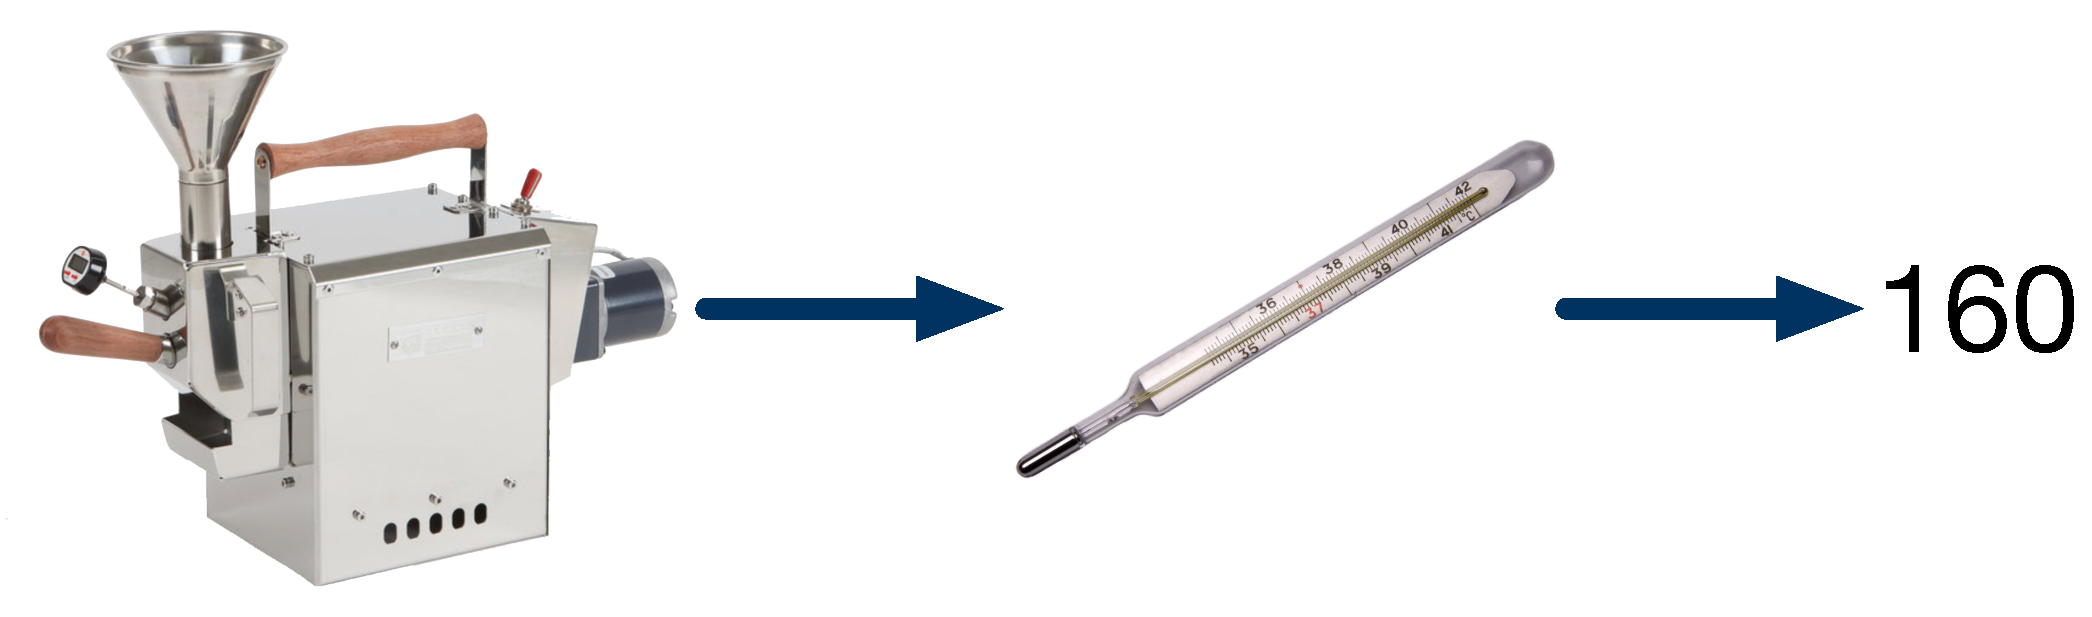
\includegraphics[width= .5 \textwidth ]{figures/roaster1}
 
  Suppose $T$ is a random variable representing the temperature of a
  roaster.
  
  What kind of object is each of the following?

  1. $g(T)$ where
  $g(t) = \begin{cases} 1, & t<150\\ 0,
    &\text{otherwise} \end{cases}$. Answer: random variable
  
  2. $R$ such that $R[T] = P(T>150)$. Answer: operator
  
  3. $T < (5/9)(T-32)$. Answer: event
  
  \note[item]{Three questions, each with three MC answers: (Event,
    Random Variable, Operator).}
\end{frame}

\subsection{Reading Call}

\begin{frame}
  \frametitle{Reading Assignment}
  Read \textit{Foundations of Agnostic Statistics}, section 1.2.2.
\end{frame}

\subsection{Discrete Random Variables}


\begin{frame}
  \frametitle{Introducing Discrete Random Variables}
  \note[item]{Random variables are quite flexible objects.}
  \note[item]{We've been using the full definition based on a probability measure, and that's a powerful idea - it can model many different things, but it's not the easiest definition to work with.}
  \note[item]{Luckily, as statisticians, we usually don't need all that power.  That's because the random variables we care about normally belong to two special classes: discrete and continuous. }
  A random variable $X$ is \textit{discrete} if its range,
  $X(\Omega) \in \R$, is a countable set.
   
  \begin{itemize}
  \item $X(\Omega)$ can be finite.
    \begin{itemize}
    \item A roll of a die: $\{1,2,3,4,5,6\}$
    \end{itemize}
  \item $X(\Omega)$ can be countably infinite.
    \begin{itemize}
    \item Edits to an article: $\{0,1,2,3...\}$
    \end{itemize}
  \end{itemize}
   
  \note[item]{You might guess the range is a discrete set in $\R$, but
    that's not quite right.  It's an uncountable set.}
\end{frame}
 
\begin{frame}[t]
  \frametitle{The Bernoulli Distribution}
   
  A Bernoulli trial is a simple (but important) discrete random
  variable.
  \begin{itemize}
  \item It can represent: 
  \begin{itemize}
\item a coin flip 
\item a decision to buy or not to buy
\item success or
    failure of experiment
\end{itemize}

  \item Convention: 1 represents success, 0 failure
  \end{itemize}
 
  \note[item]{$\Omega = {H,T}$} \note[item]{$P(H) = p$, $P(T) = 1-p$}
  \note[item]{Let $X(H) = 1$, $X(T) = 0$.}  \note[item]{$P(X=1) = p$,
    $P(X=0) = 1-p$}
\end{frame}
 
  
\begin{frame}[t]
  \frametitle{The Probability Mass Function (PMF)}
   
  A function that gives the probability that a discrete random
  variable equals each number in $\R$

  \begin{itemize}
  \item $f_X(x) = P(X = x)$
  \end{itemize}
  \vspace{.5cm} 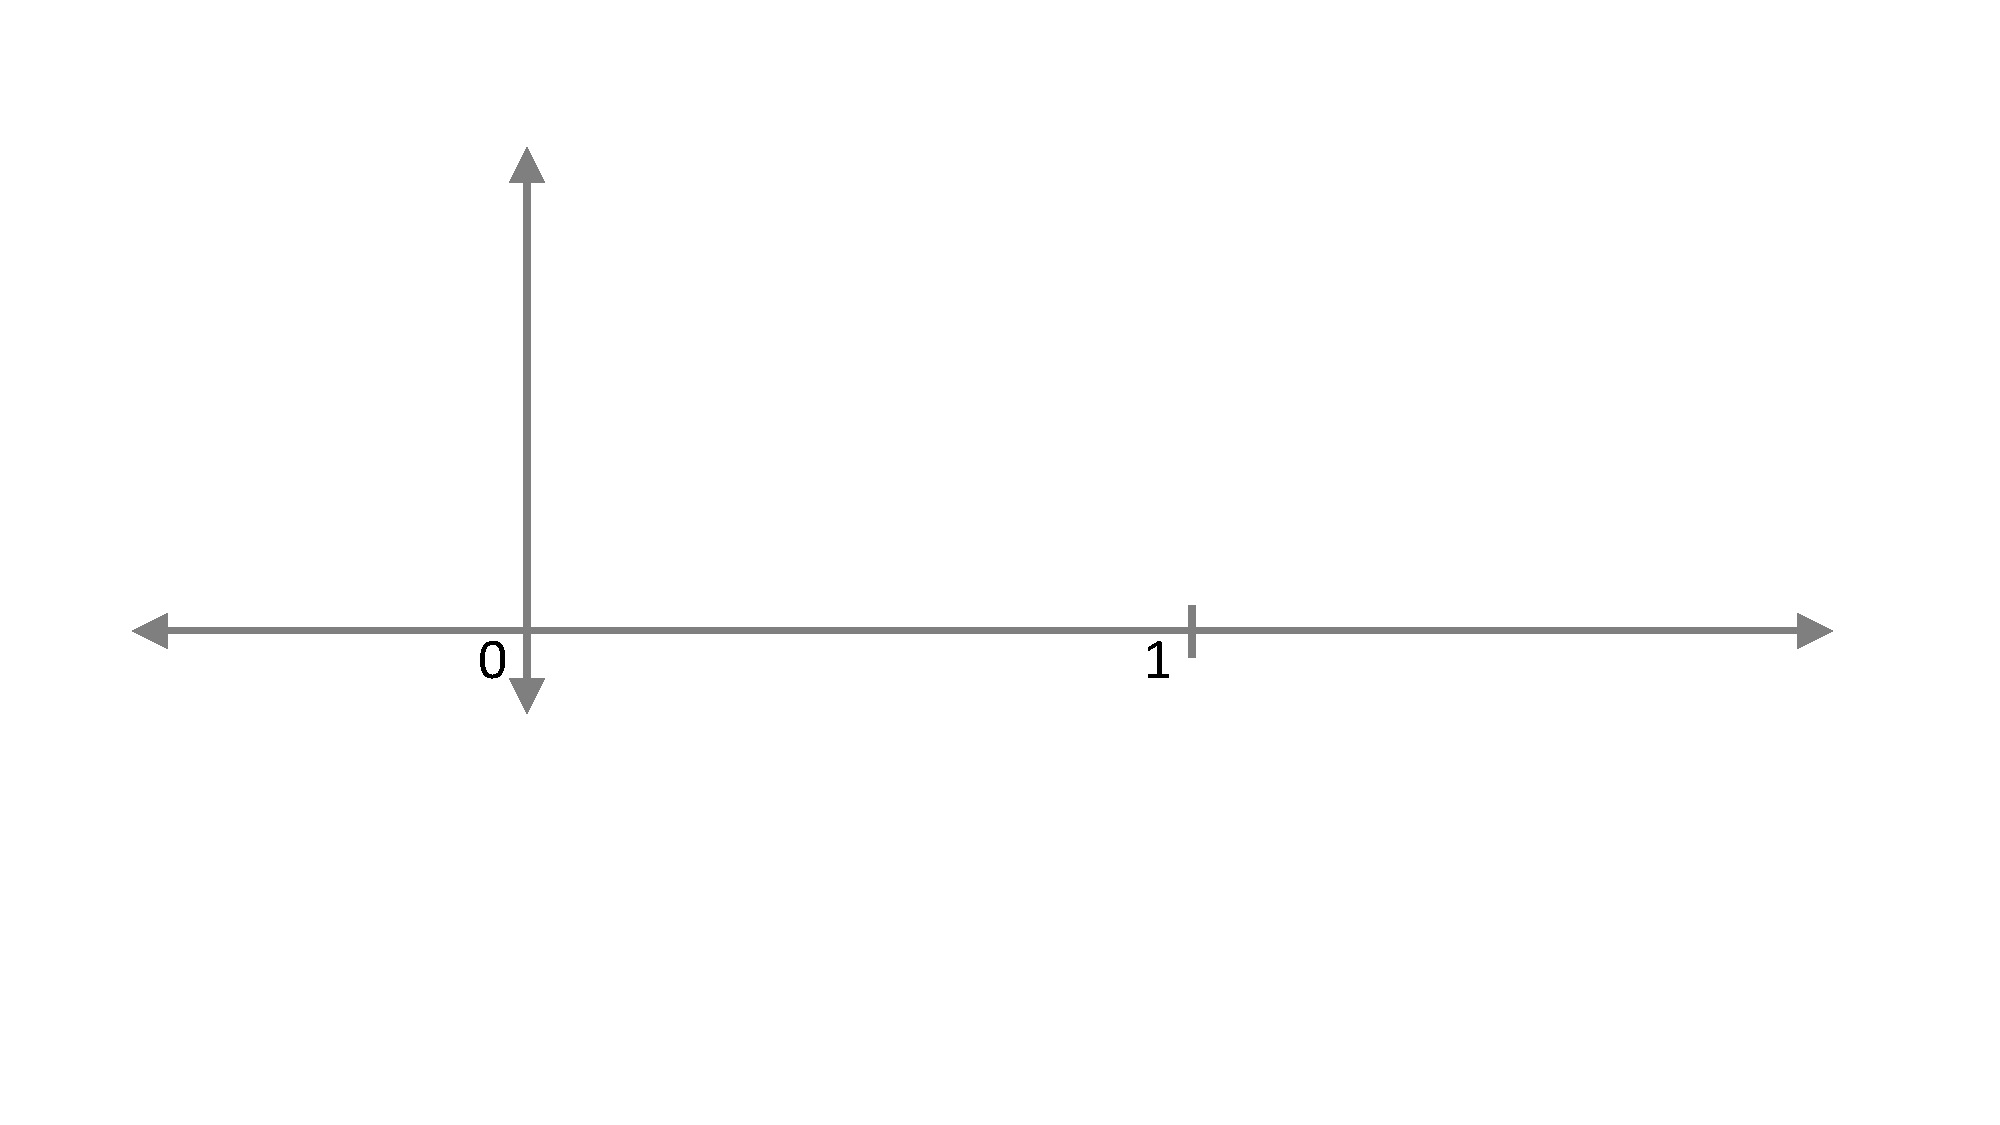
\includegraphics[width= \textwidth ]{figures/axes}
 
  \note[item]{sketch the probability distribution for the Bernoulli
    trial} \note[item]{write out pdf with cases}
\end{frame}
 
 
\begin{frame}
  \frametitle{Key Properties of the PMF}

\begin{block}{Theorem}
  For a discrete random variable $X$ with pmf $f$, 
  
  \begin{enumerate}
  \item For all $x \in \R$, $f(x) \geq 0$.
  \item $\sum_{x \in X(\Omega)} f(x) = 1$.
  \end{enumerate}
\end{block}
\note[item]{$f(x) = P(X=x)$ and $P(anything)\geq 0$ by axiom 1}
\note[item]{$\sum_{x \in X(\Omega)} P(X=x) = P( \cup_{x \in X(\Omega)}
  (x = X) ) = P(x \in X(\Omega)) = 1$} \note[item]{Hopefully you find
  these intuitive.  The values of $f$ are probabilities, so they have
  to follow all the axioms of probability} \note[item]{So not
  surprising, but these are great sanity checks.  My advice is that
  when you need to answer a question with a pmf, you check these two
  things.}
\end{frame}
 
 
\begin{frame}
  \frametitle{Computing Other Event Probabilities from the PMF}

\begin{block}{Theorem: The PMF fully characterizes a discrete RV}
  For a discrete random variable $X$ with pmf $f$, if $D \subseteq \R$,
  $$  P(X \in D) = \sum_{x \in X(\Omega) \cap D } f(x).$$
\end{block}
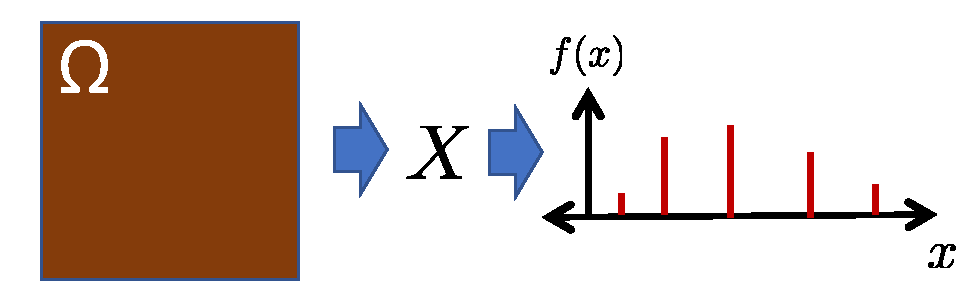
\includegraphics[width= \textwidth]{figures/pmf_to_events} Take-away:
The pmf contains \textit{all} the information about the probability
distribution of $X$.
\end{frame}
 
\subsection{Reading: Cumulative Distribution Functions}

\begin{frame}
  \frametitle{Reading Assignment}
  Read \textit{Foundations of Agnostic Statistics}, section 1.2.3.
\end{frame}
 
 
\subsection{Lightboard: The Cumulative Distribution Function}
 
\begin{frame}

  \frametitle{The Cumulative Distribution Function}
  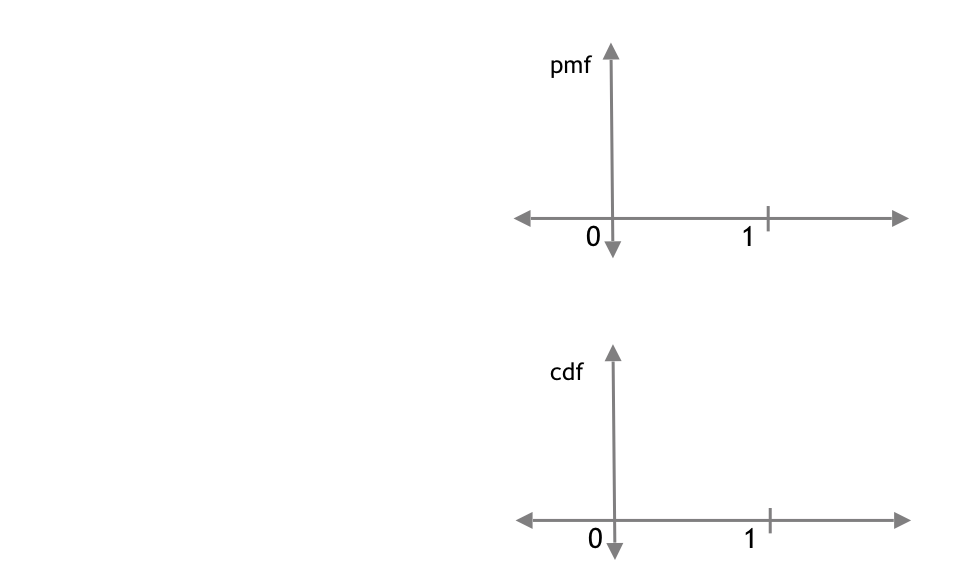
\includegraphics[width=\textwidth
  ]{figures/cdf_axes}
\end{frame}

\begin{frame}
  \frametitle{The Cumulative Distribution Function (Solution)}
  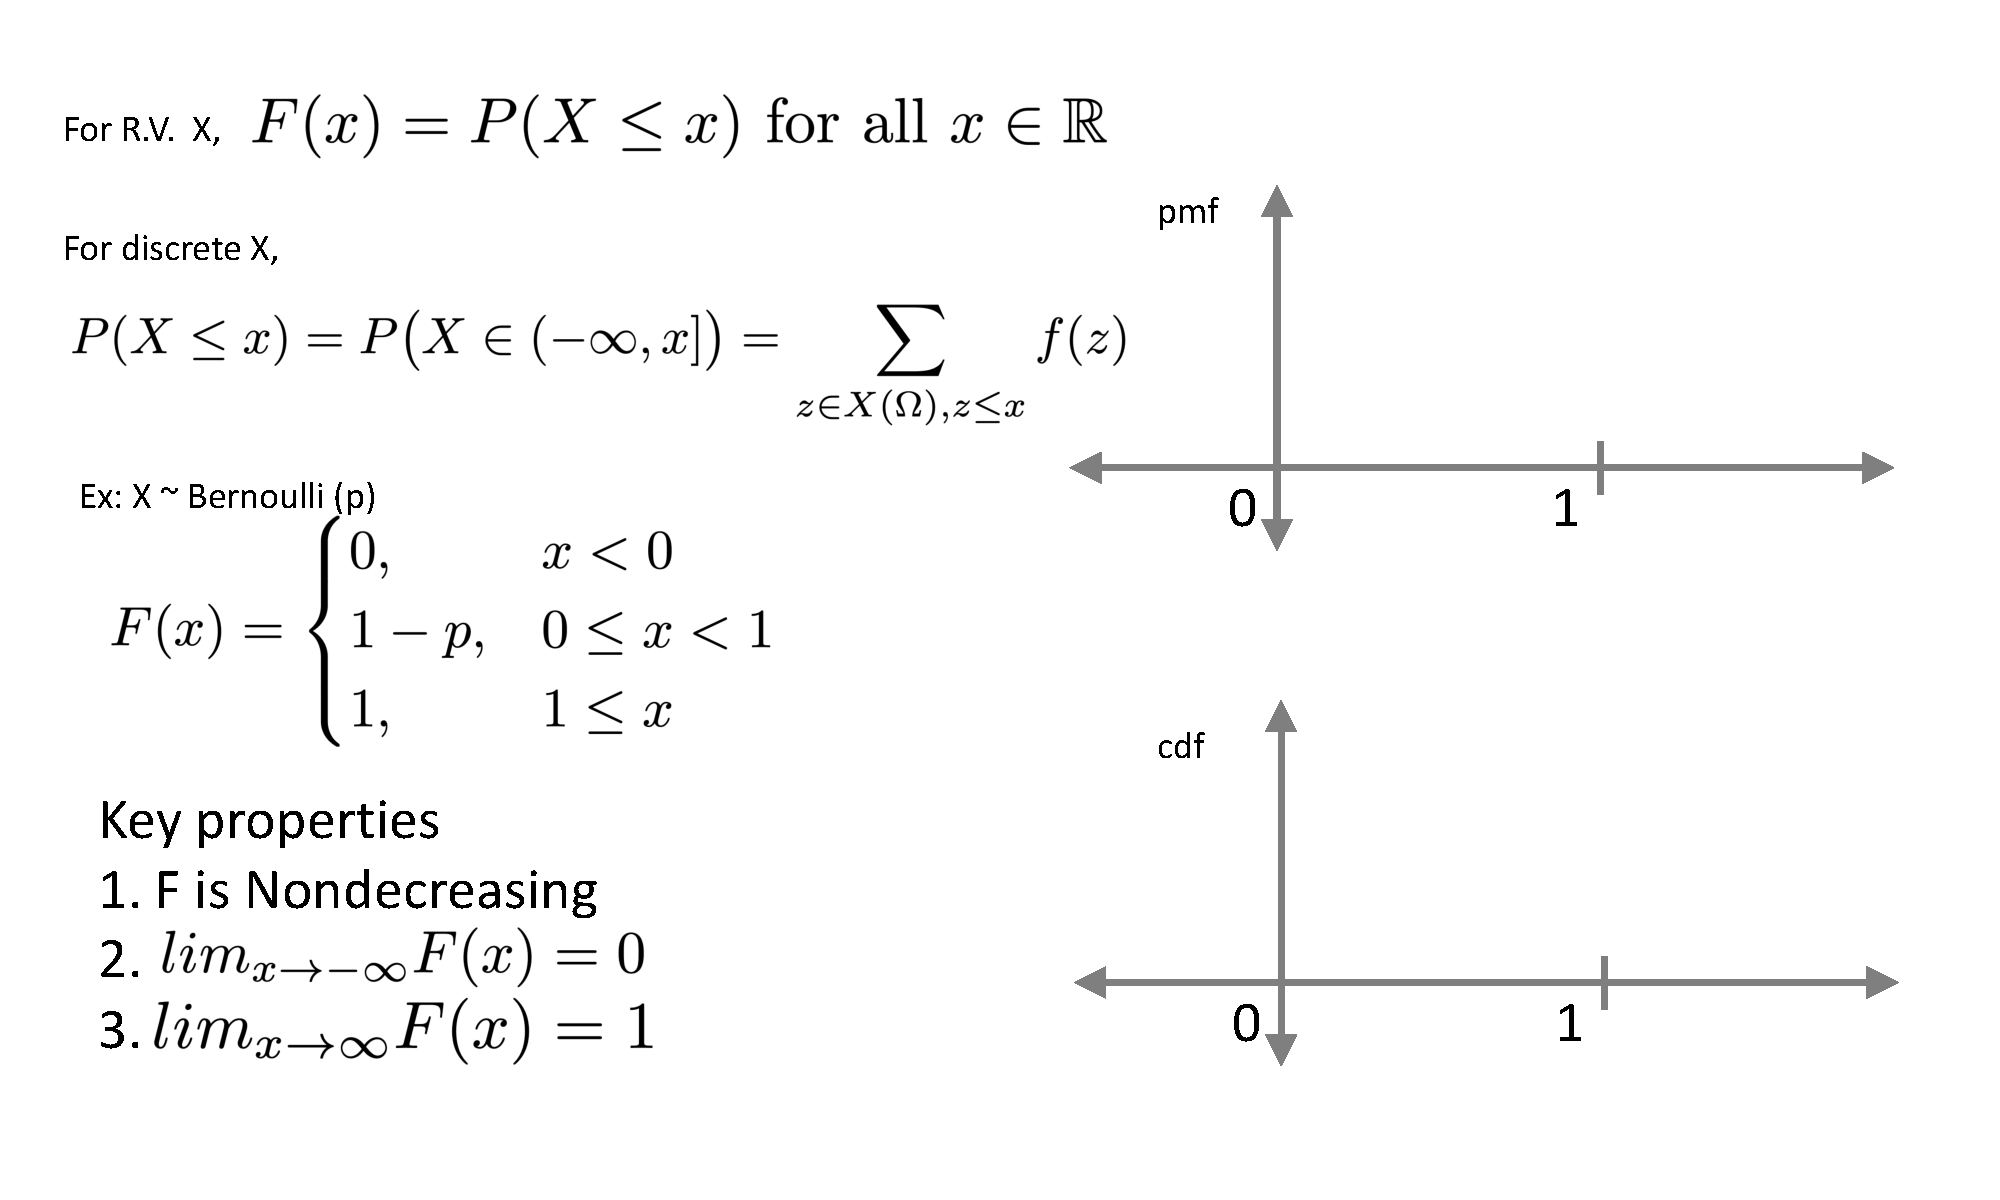
\includegraphics[width= \textwidth
  ]{figures/cdf_axes_key}
  \note[item]{You already know that a PMF fully describes the distribution of a discrete random variable.}
\note[item]{There is another tool that's really important for describing distributions, and that's the CDF}
  \note[item]{I have to admit, when you're learning, the CDF is less intuitive than the PMF.  but
    there is one big advantage. }
    \note[item]{ The CDF completely specifies the
    distribution of ANY RV, not just a discrete one.  It doesn't place any assumptions on the random variable.  so we like to write theorems that use the CDF, because those are as general as possible.}
\end{frame}

\subsection{Continuous Random Variables}

\begin{frame}
  \frametitle{Motivation for Continuous Random Variables}
  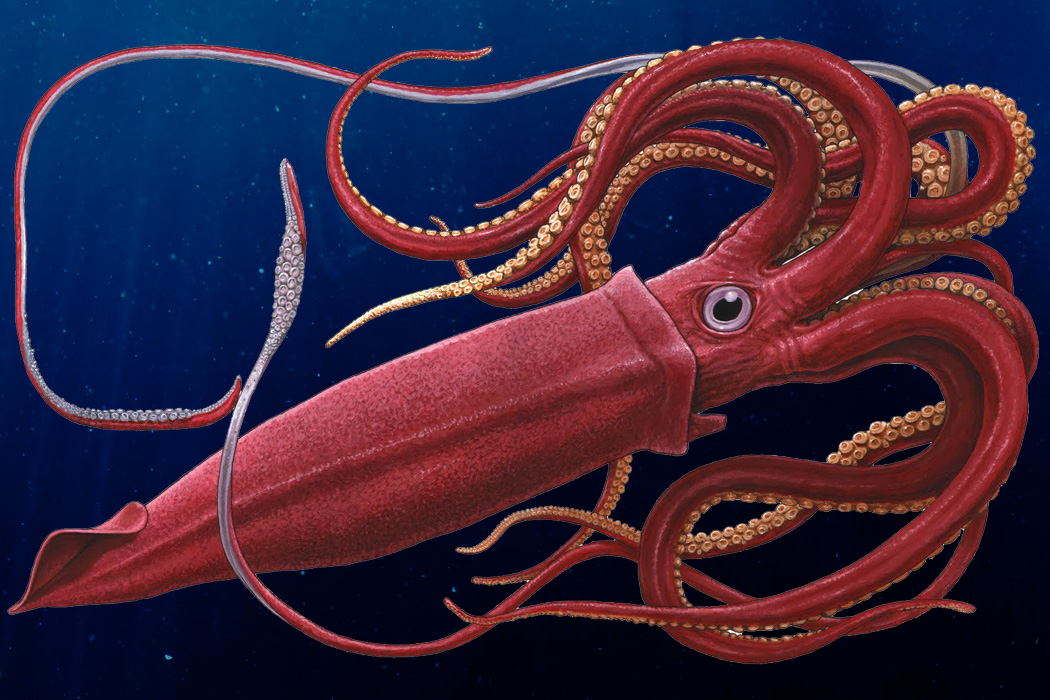
\includegraphics[width=\textwidth ]{figures/squid} \note[item]{Let's
    say you're studying a rare species of giant squid.  I ask you,
    what's the probability that a specimen is exactly 6 meters long?}
  \note[item]{You might estimate that maybe 20\% are between 5.5 and
    6.5 meters.}  \note[item]{But my question is what's the
    probability that a squid is exactly 6 meters.}  \note[item]{To
    within 1 mm?  to within 1 nanometer?}  \note[item]{You can quickly
    see that the probability of 6 meters with zero error is actually
    0.}
  
\end{frame}
 
 
\begin{frame}
  \frametitle{Motivation for Continuous Random Variables}
  
  \begin{tabularx}{\textwidth}{ *{6}{X} }
    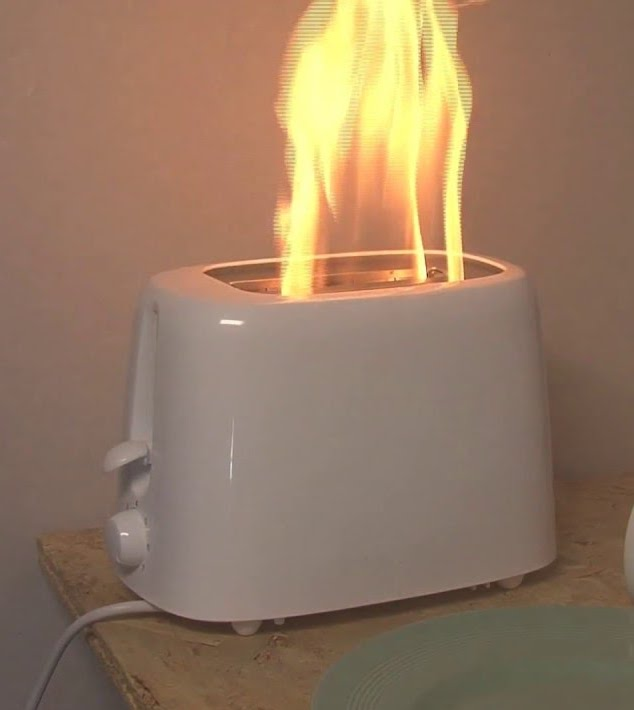
\includegraphics[width=  .3  \textwidth]{figures/toaster}   &   &  \\
  \end{tabularx}
  
  \note[item]{There are a lot of other variables that also take on a
    continuum of values.}  \note[item]{force until a piece of
    equipment breaks,}
\end{frame}

\begin{frame}
  \frametitle{Motivation for Continuous Random Variables}
  \begin{tabularx}{\textwidth}{ *{6}{X} }
    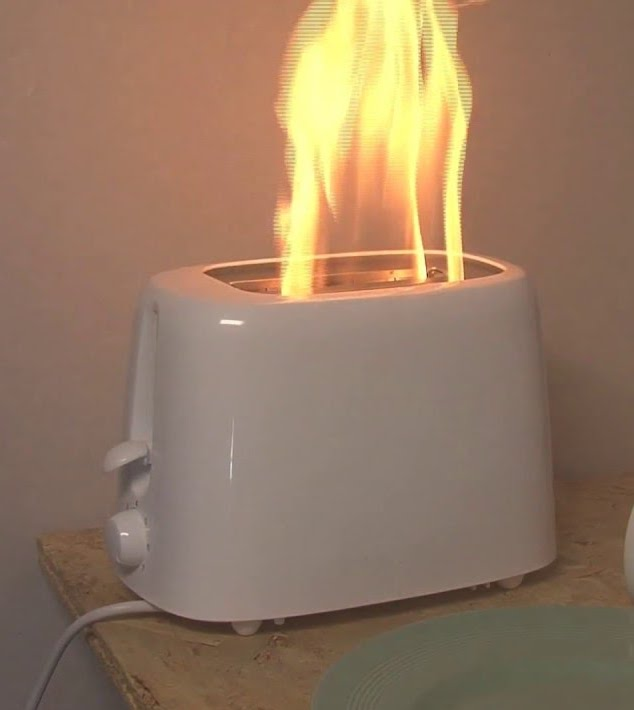
\includegraphics[width=  .3  \textwidth]{figures/toaster}   & 
                                                                  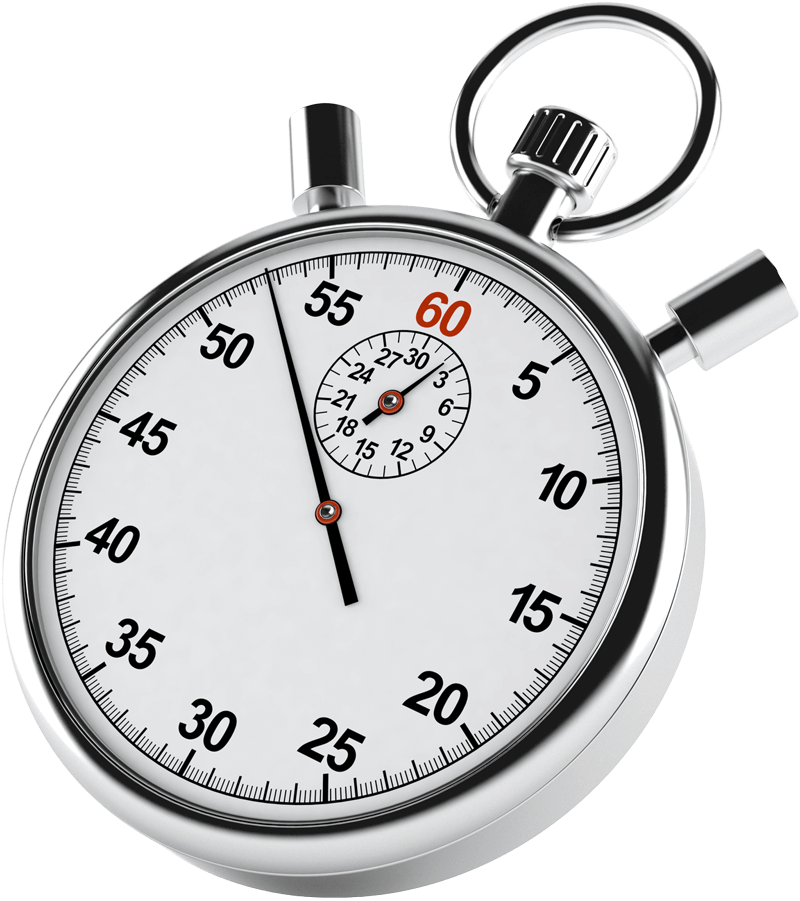
\includegraphics[width=  .3 \textwidth ]{figures/clock}  & 
    \\
  \end{tabularx}
  \note[item]{ time between customer visits}
\end{frame}


\begin{frame}
  \frametitle{Motivation for Continuous Random Variables}
  \begin{tabularx}{\textwidth}{ *{6}{X} }
    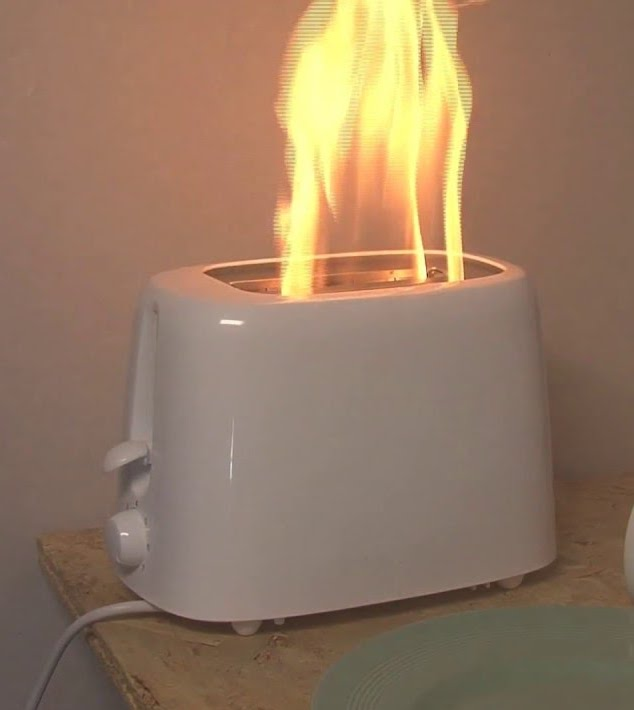
\includegraphics[width=  .3  \textwidth]{figures/toaster}   & 
                                                                  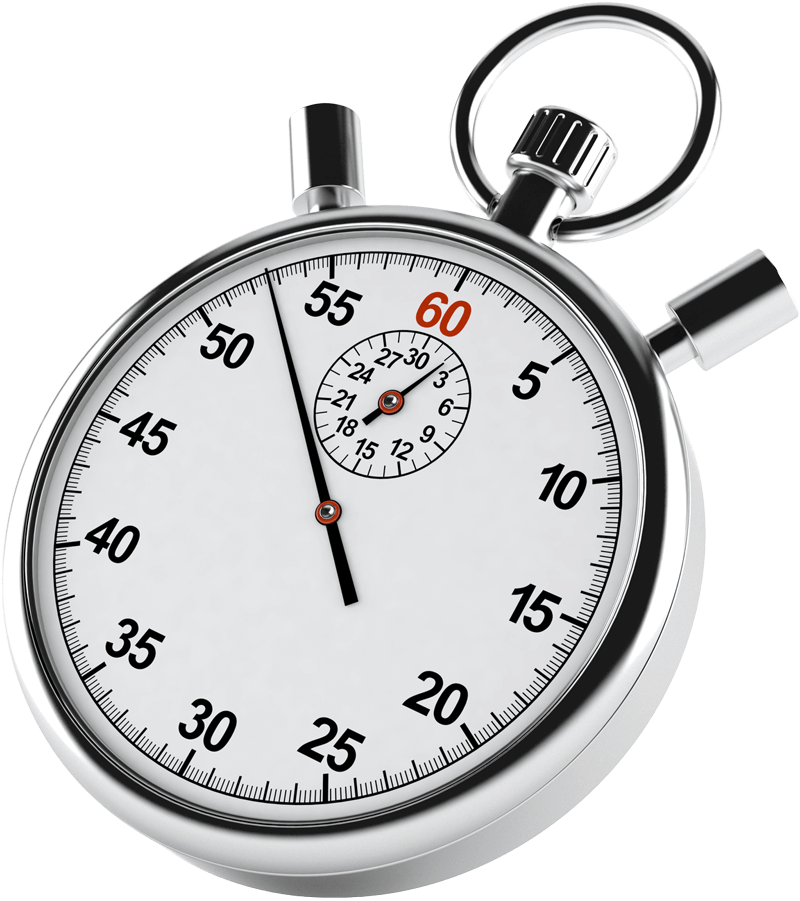
\includegraphics[width=  .3 \textwidth ]{figures/clock}  & 
                                                                                                                             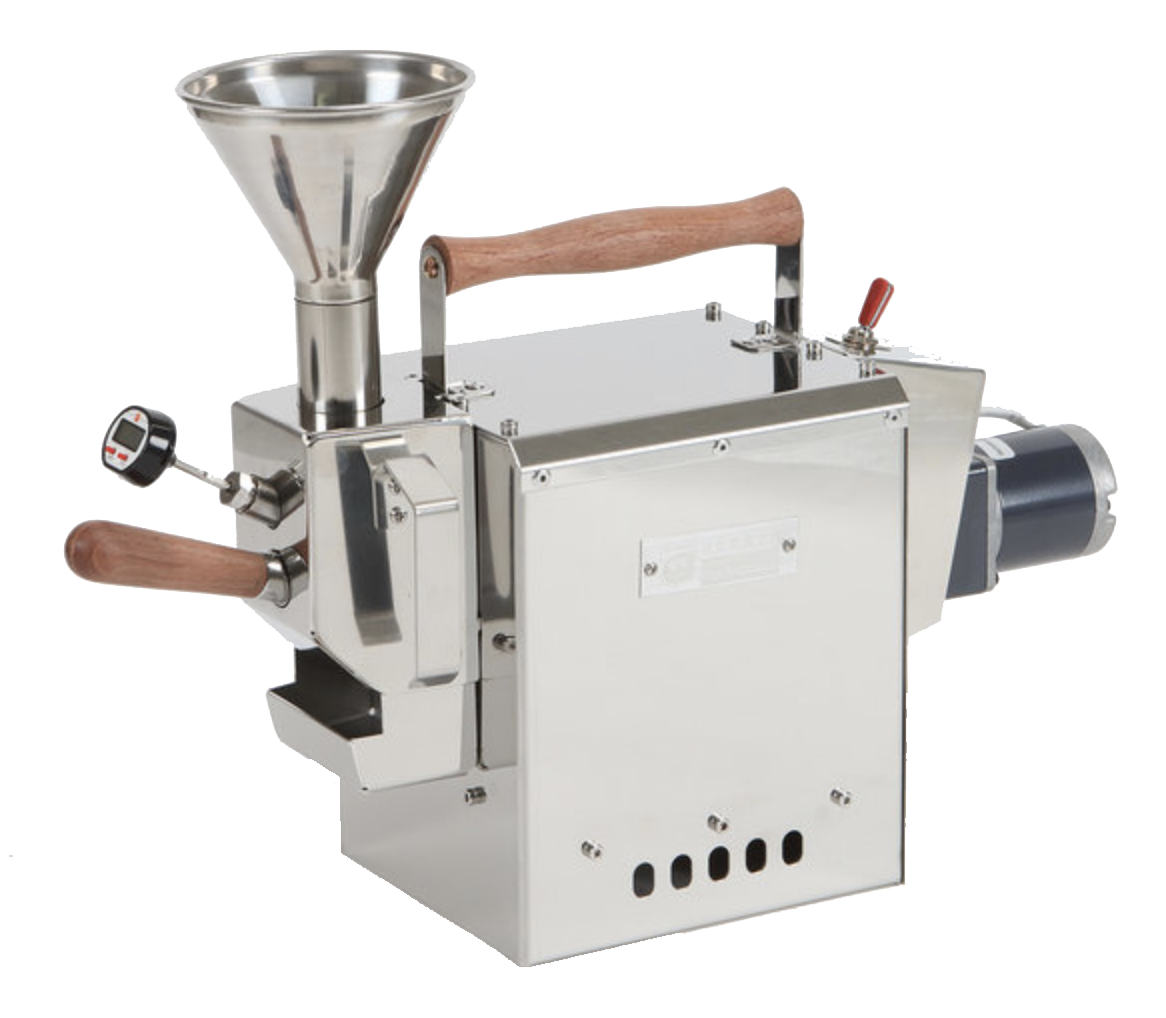
\includegraphics[width=  .3  \textwidth ]{figures/roaster} \\
  \end{tabularx}
  
  \note[item]{temperature of a coffee roaster...}  \note[item]{How do
    we model these situations as statisticians?}  \note[item]{We could
    pretend that they are discrete.  Or we could focus on what we
    measure with our instrument.  Since we have finite precision, the
    set of numbers we can write down is countable.  But that might
    feel like cheating, and in any cse, it actually makes the math
    really complicated.  Instead, we prefer to use what we call
    continuous random variables..}
\end{frame}


\begin{frame}
  \frametitle{The Probability Density Function}
  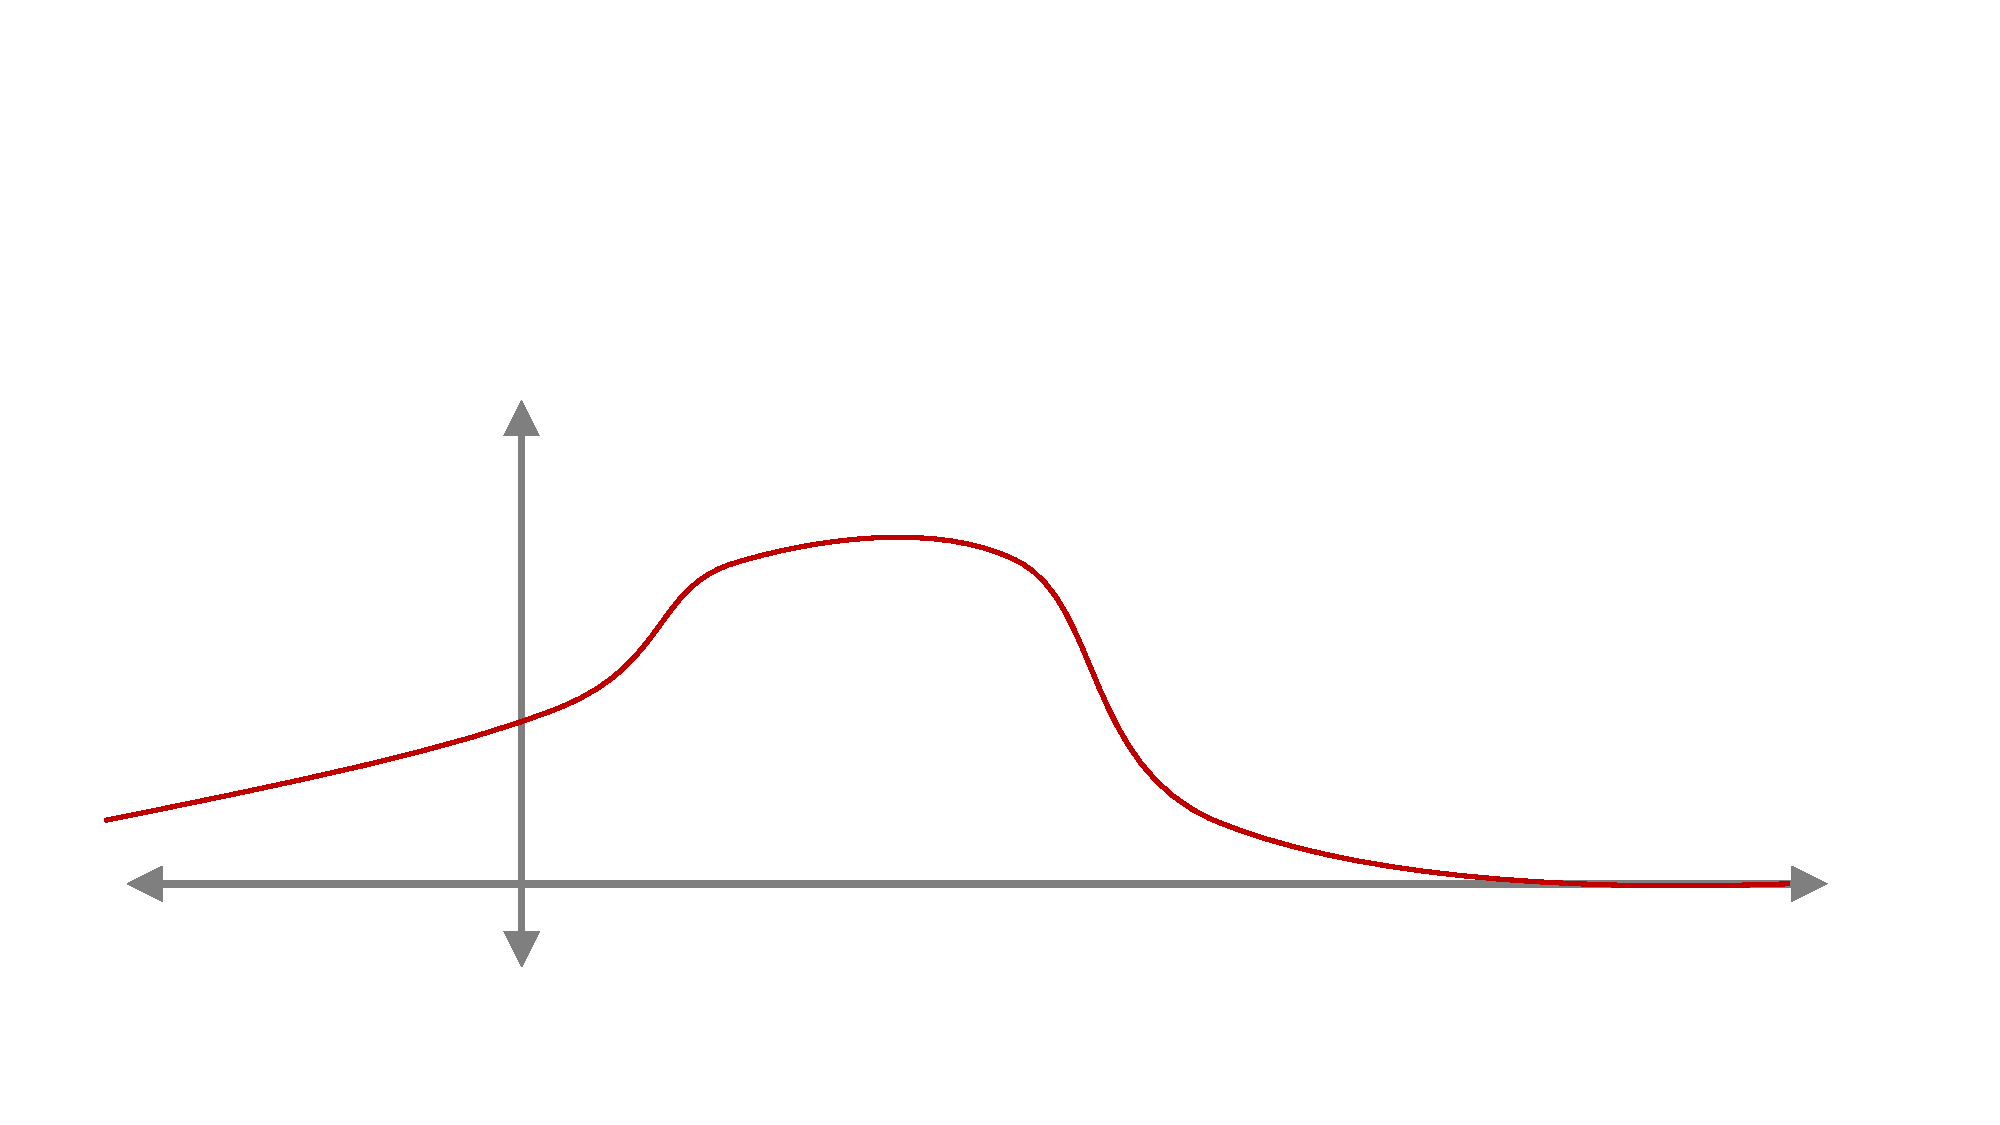
\includegraphics[width= \textwidth]{figures/density} \note[item]{The
    core idea behind continuous random variables is a probability
    density function} \note[item]{The purpose is to show how
    probability is spread out over the range of possible values}
  \note[item]{The probability of any one point is zero}
  \note[item]{But if you have a range, what you do is you integrate
    under the density to get the probability} \note[item]{Draw
    interval and indicate area....}  \note[item]{This gives us a
    principled way to talk about probabilities over a continuum of
    values}
\end{frame}



\subsection{Reading: Continuous Random Variables}

\begin{frame}
  \frametitle{Reading: Continuous Random Variables}
  Read \textit{Foundations of Agnostic Statistics}, section 1.2.4.
\end{frame}

\subsection{Properties of Continuous Random Variables}

\begin{frame}
  \frametitle{Continuous Random Variables}
  \begin{block}{Definition}
  A random variable $X$ is \textit{continuous} if there exists a non-negative function $f:\R \rightarrow \R$ such that the cdf of $X$ is
  $$F(x) = \int_{-\infty}^x f(u) du \text{, for all } x \in \R$$
  \end{block}
    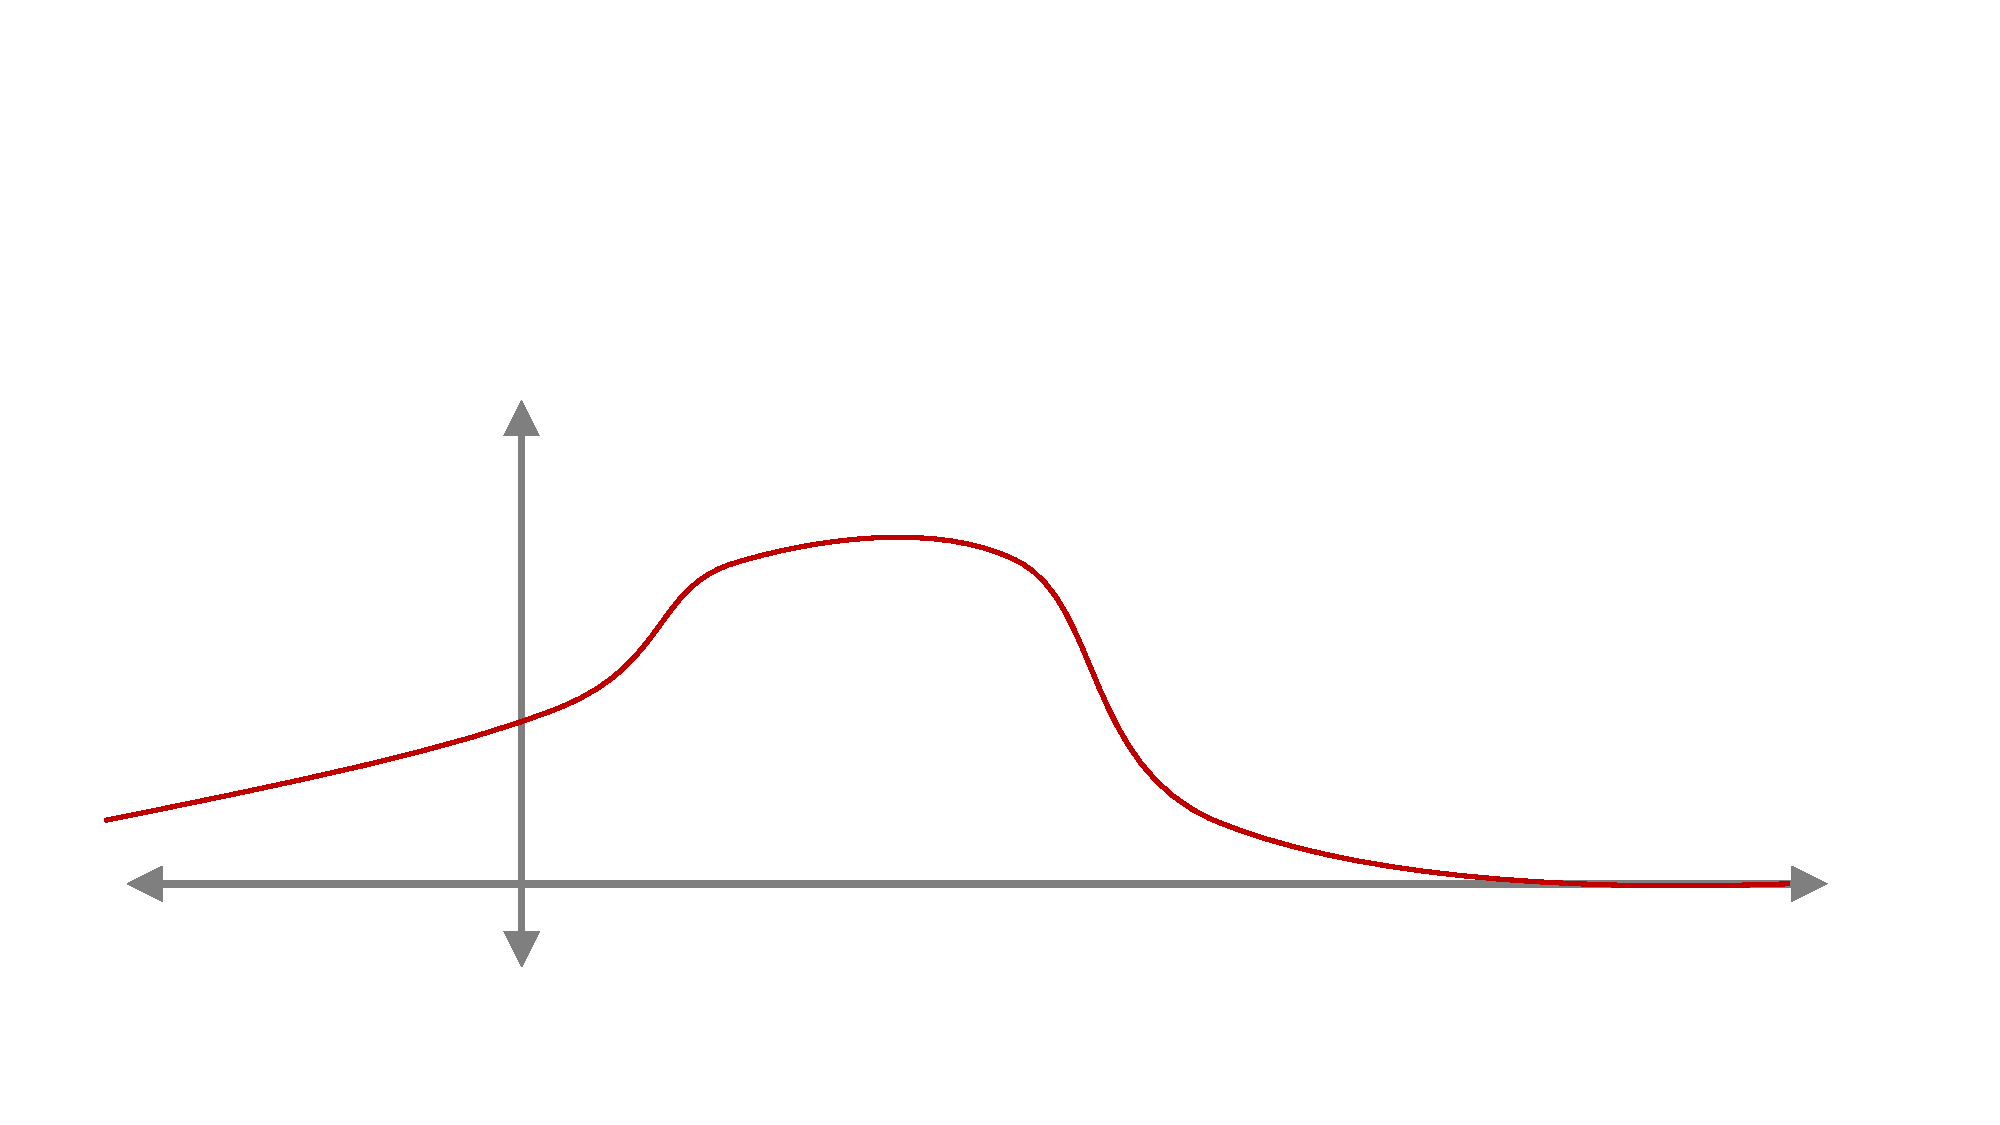
\includegraphics[width= \textwidth]{figures/density} 

  \note[item]{How do we define a continuous random variable?  It's a random variable that has a probability density function}
  \note[item]{We know that every random variable has a CDF.  for a continuous random variable, the pdf determines the cdf.  How do you get the CDF from the pdf?}
  \note[item]{The CDF at some point x, is the probability the RV is less than or equal to x.}
  \note[item]{How do we get that?  we integrate from -infinity to x}
\end{frame}

\begin{frame}
  \frametitle{Characterizing Continuous Random Variables}
  
  \begin{block}{Deriving the PDF from the CDF}
  For a continuous random variable with cdf $F$, the probability density function of $X$ is
  $$f(x) = \frac{dF(u)}{du} \Bigg|_{u=x} \text{, for all } x \in \R$$
  \end{block}
      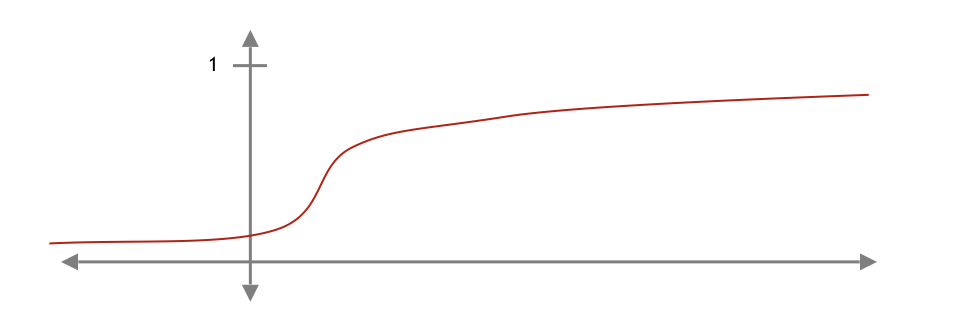
\includegraphics[width= \textwidth]{figures/cdf} 
  \note[item]{If you take an integral to get from the pdf to CDF, how do you go the other way?}
  \note[item]{This is really just the fundamental theorem of calculus: take a derivative.}
  \note[item]{think about the the cdf at some point x, this is $P(X < x)$}
  \note[item]{Then move to the right by some tiny dx.  the cdf now represents $P(X<x+dx)$}
  \note[item]{So the difference is just $P(x < X < x + dx)$.  it's the probability x is in this tiny rectangle.}
  \note[item]{That's how quickly we're adding in probability.  If we divide by the width of the rectangle, we get the slope, and that's exactly the probability density.}
\end{frame}


\begin{frame}
  \frametitle{}
  \note[item]{Here are two important properties of pdfs.}
  \note[item]{Use these as sanity checks.  when you write down a pdf, see if these properties hold.}
  \note[item]{If they don't, you've done something wrong.}
  \begin{block}{Properties of Probability Density Functions}
  For a continuous random variable $X$ with pdf $f$,
  \begin{enumerate}
  \item For all $x\in \R$, $f(x) \geq 0$.
  \item $\int_{-\infty}^\infty f(x)dx = 1$.
  \end{enumerate}
  \end{block}
\end{frame}


\begin{frame}[t]
  \frametitle{Support}
  \begin{block}{Definition}
  For a random variable $X$ with pmf or pdf $f$, the \textit{support} of $X$ is
  $$\text{Supp}[X] = \{x \in \R : f(x) > 0 \}$$
  \end{block}
  \note[item]{This will be helpful when we discuss continuous distributions.  we'll usually assume we're in the support, because we don't want to divide by zero.}
\end{frame}



 
\subsection{Uniform Random Variables}

\begin{frame}
  \frametitle{Uniform Random Variables}

  \textbf{Note: This is a placeholder for a video that we're going to
    re-use from:} Use the old video 3.9 Uniform Random Variables -
  only the start through 6.12, before I start talking about
  expectation.

\end{frame}

\subsection{Normal Random Variables}

\begin{frame}  
Use the old video 3.10 The Normal Distribution
\end{frame}






%Begin Section 2.16 Edits

\subsection{Normal Random Variables}

\begin{frame}
  \frametitle{The Normal Distribution}
  \textbf{The most important distribution in statistics}
  \begin{itemize}
    \item The variables measured don't always come directly from a normal distribution
    \begin{itemize}
      \item Human height has a close-to-normal distribution--so do anthropometric measurements on fossils, reaction times in psychological experiments, etc.
      \item Most variables deviate from a normal distribution
    \end{itemize}
    \item We'll see how the normal distribution pops up as a consequence of basic mathematical laws
    \item A famous theorem is the \textbf{Central Limit Theorem}. Many of our statistical tests depend on this theorem, and it tells us when certain distributions will approach a normal distribution
  \end{itemize}
\end{frame}

\begin{frame}
  \frametitle{The Normal Distribution equation}
  A continuous rv $X$ is said to have a \textbf{normal distribution} with parameters $\mu$ and $\sigma$ (or $\mu$ and $\sigma^{2}$), where $-\infty < \mu < \infty$ and $ 0 < \sigma$, if the pdf of $X$ is:
  
  \begin{equation}
     f(x; \mu, \sigma) = \frac{1}{\sqrt{2\pi\sigma^{2}}}
     e^{-(x-\mu)^{2}/(2\sigma^{2})},
     -\infty < x < \infty
  \end{equation}
  This is the equation for the density function of a normal distribution
\end{frame}

\begin{frame}
  \frametitle{The Normal Distribution equation}
  
  \begin{equation}
     f(x; \mu, \sigma) = \frac{1}{\sqrt{2\pi\sigma^{2}}}
     e^{-(x-\mu)^{2}/(2\sigma^{2})},
     -\infty < x < \infty
  \end{equation}
  
  \begin{itemize}
    \item There are two parameters, $\mu$ and $\sigma$
    \begin{itemize}
      \item There is an entire family of normal distributions
    \end{itemize}
    \item It can be shown that $E(x)=\mu$ and $V(X)=\sigma^{2}$, so the parameters are the mean and the standard deviation of $X$
    \item The statement that $X$ is normally distributed with parameters $\mu$ and $\sigma^{2}$ is often abbreviated $X \sim N(\mu, \sigma^{2})$
  \end{itemize}
\end{frame}

\begin{frame}
  \frametitle{Normal Curve Examples}
  \begin{center}
      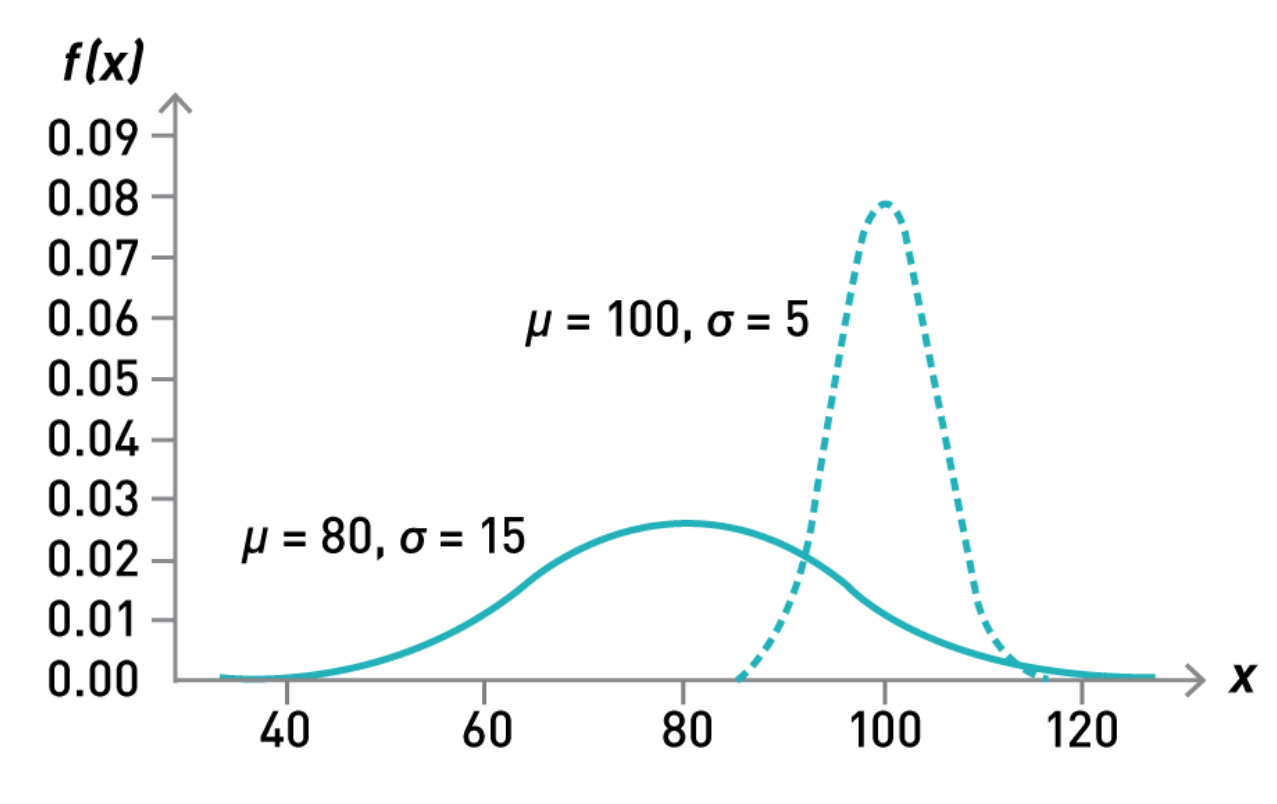
\includegraphics[width=.5\linewidth]{figures/normal_curve.png}
  \end{center}
  \begin{itemize}
      \item These are normal curves with different $\mu$ and $\sigma$
      \item Each curve is symmetric around its mean
      \item $\mu$ is both the mean and the median, changing it moves the curve left or right
      \item $\sigma$ is also called the scale parameter, since it stretches the curve horizontally
  \end{itemize}
\end{frame}

\begin{frame}
  \frametitle{The Standard Normal Distribution}
  \begin{itemize}
      \item Often, we need to select one representative distribution out of the normal family
      \item Typically, we choose $\mu=0$ and $\sigma=1$
      \begin{itemize}
          \item This is called the \textit{standard normal distribution}, also called a \textit{z-distribution}
          \item It is also denoted by a capital Z
          \item We can write the pdf of Z:
      \end{itemize}
  \end{itemize}
  \begin{equation}
      f(z; 0, 1)= \frac{1}{\sqrt{2\pi}}e^{-z^{2}/2},
      -\infty < X < \infty
  \end{equation}  
  \begin{itemize}
      \item The cumulative distribution of Z is often written as $\phi(z)$
  \end{itemize}
\end{frame}

\begin{frame}
  \frametitle{Standardizing a Normal Variable}
  \begin{itemize}
      \item Suppose we have a normal variable that is not standard normal $X \sim N(\mu, \sigma^{2})$
      \begin{itemize}
          \item We want to simplify our computations
      \end{itemize}
      \item We can compute the random variable $(X-\mu) / \sigma$
      \begin{itemize}
          \item This new variable has a standard normal distribution
          \item This can make it easier to perform tests using the variable
      \end{itemize}
      \item Any probabilities involving $X$ can be expressed in terms of areas under the z-distribution
  \end{itemize}
\end{frame}

\begin{frame}
  \frametitle{Standardizing a Normal Variable (cont.)}
  These are easy to compute in statistical software
  \begin{center}
    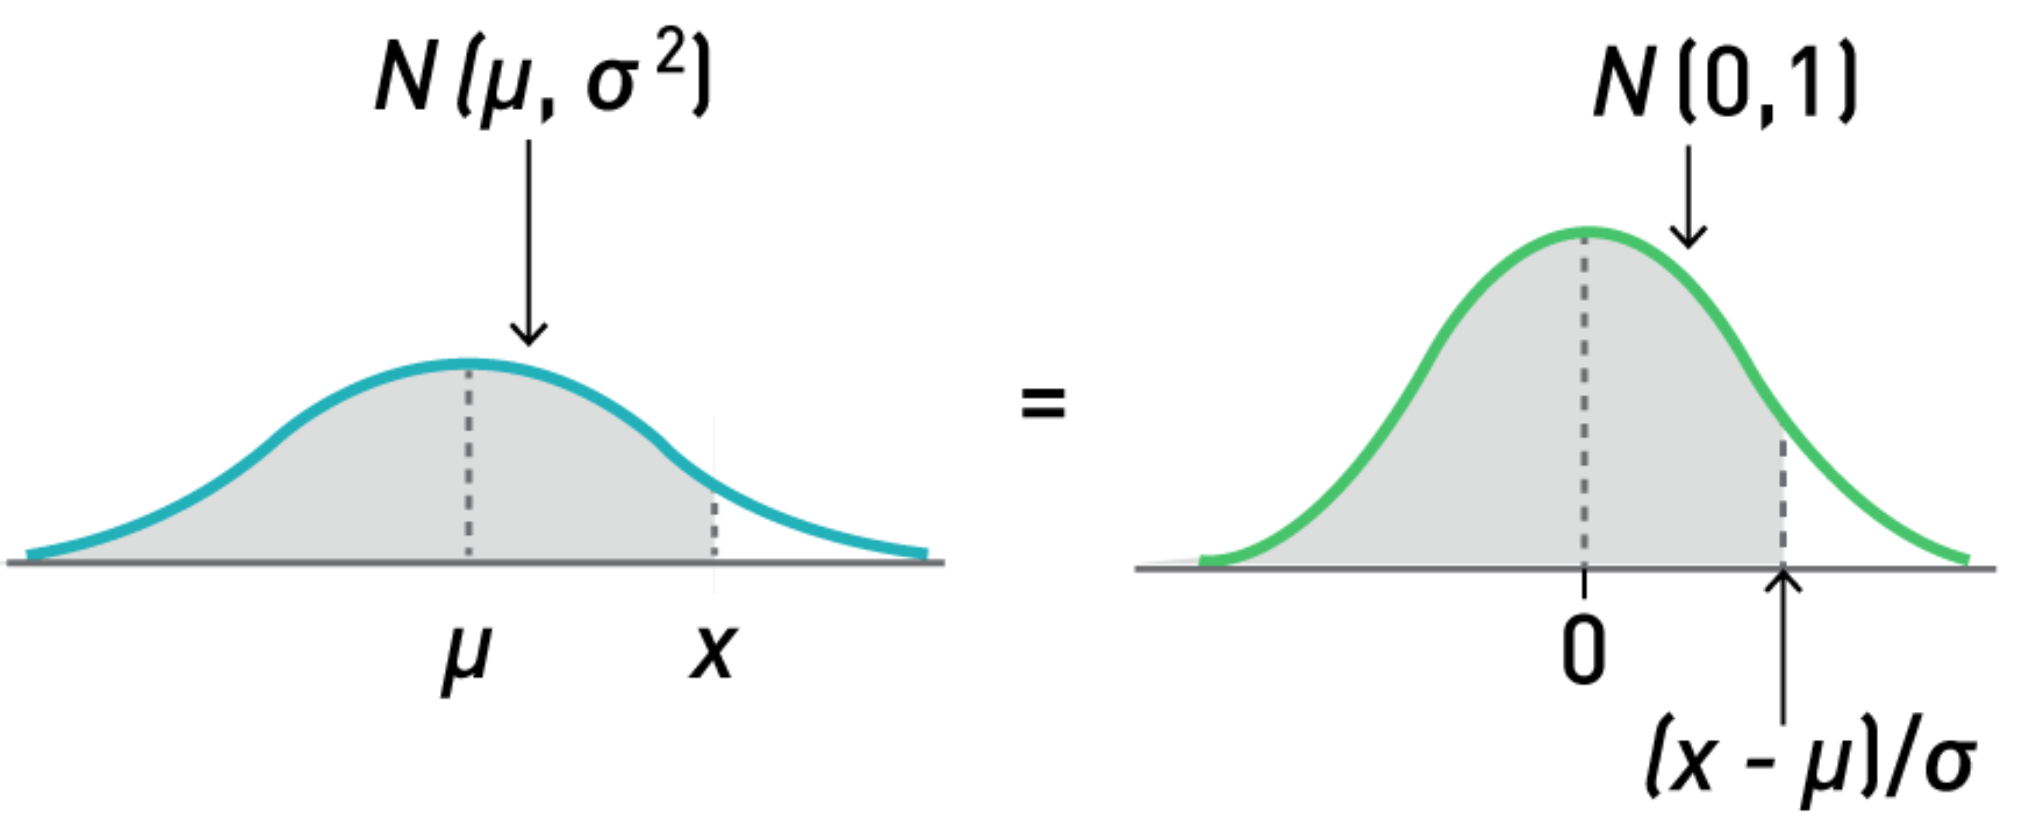
\includegraphics[width=0.9\linewidth]{figures/standardizing_normal_variable.png}
  \end{center}
\end{frame}

\begin{frame}
  \frametitle{Properties of the Normal Distribution}
  \begin{center}
      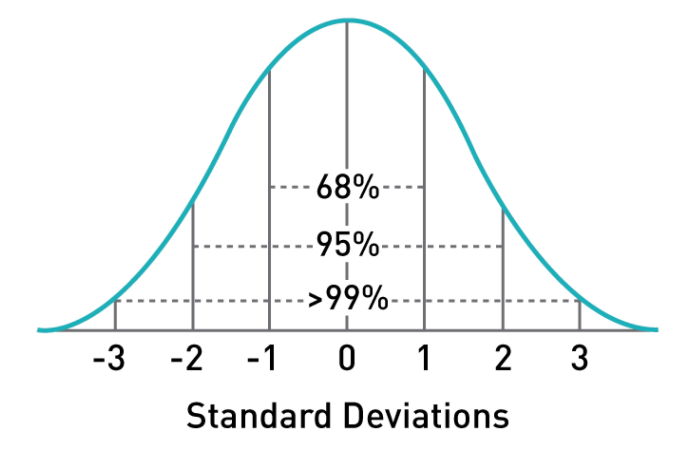
\includegraphics[width=0.5\linewidth]{figures/properties_normal_distribution.png}
  \end{center}
  This picture shows certain areas under a normal curve
  \begin{itemize}
      \item 68\% of the area is within 1 standard deviation of the mean
      \item 95\% is within 2 standard deviations
      \item 99.7\% is within 3 standard deviations
  \end{itemize}
\end{frame}

\begin{frame}
  \frametitle{Properties of the Normal Distribution (cont.)}
  \begin{exampleblock}{Important Rules of Thumb (helpful to memorize)}
    \begin{enumerate}
        \item It can be helpful when you have a variable that is approximately normally distributed
        \item You would expect about 68\% of values to be within 1 standard deviation
        \item Very few values are more than 2 standard deviation away from the mean (this will be important when we look at hypothesis testing)
    \end{enumerate}
  \end{exampleblock}
    
\end{frame}

\section{Part 2: Joint Distributions} 

\subsection{Joint Distributions}

\begin{frame}
  \frametitle{Introducing Joint Distributions}

  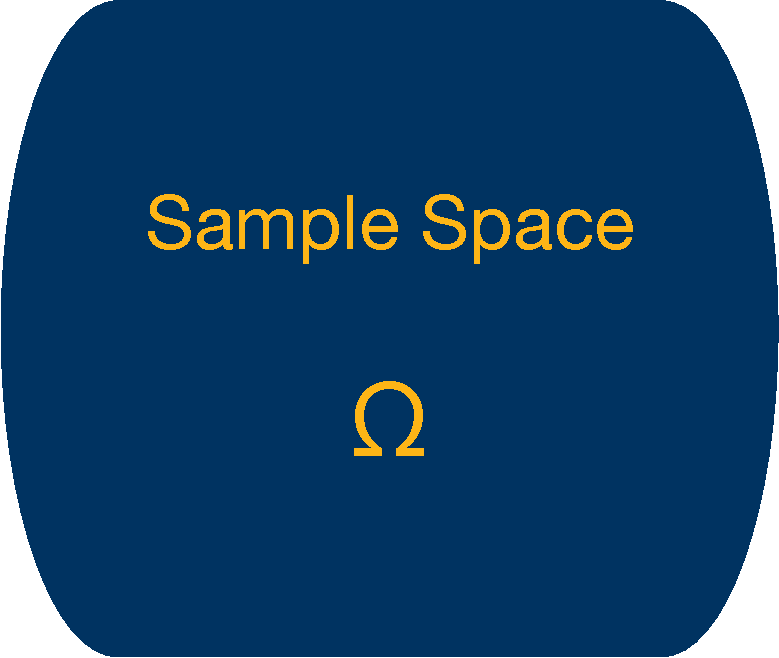
\includegraphics[width= .4\textwidth ]{figures/sample_space}

  \note[]{
    \begin{itemize}
    \item Suppose that you're consulting for a car dealer to build a
      statistical model of a customer -- ``Will \textit{this} customer
      buy a car?
    \item You begin by defining a random variable $B$, that takes the
      value $B=1$ if the customer buys, and $B=0$ if they don't.
    \item Without any additional informaiton, your best guess is no
      better than the historical average sales -- and the dealer
      already has that! You need to do \textit{better} to be valuable.
      \begin{itemize}
      \item Number of test drives
      \item Size of family
      \end{itemize}
    \item No problem! Just make new random variables!
    \end{itemize}
  }
\end{frame}

\begin{frame}
  \frametitle{Introducing Joint Distributions}
  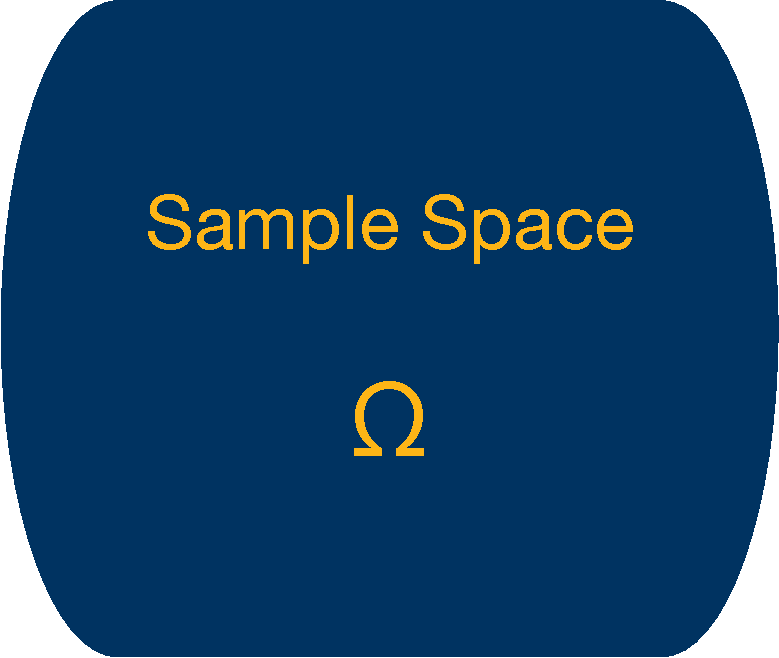
\includegraphics[width= .4\textwidth ]{figures/sample_space}
  
  \note[item]{Because we have this separate probabiliity space, it's
    easy to define a new random variable D, that maps from $\Omega$ to
    $\R$.  D represents how many cars the customer test drives, 0,1,
    or 2 - you only have 2 models to keep it simple}
 
  \note[item]{One way to look at this is we have Probability Measure P
    over the sample space.  Through these random variables, you could
    show that this induces a probability measure over $\R^2$ - that's
    what we call a joint distribution.}

  \note[item]{We're going to spend a lot of time working with sets of
    random variables to do a variety of useful things.  But right now,
    we're really starting with just the basics - what are ways of
    defining and describing joint distributions? }
\end{frame}

\subsection{Reading Assignment}

\begin{frame}
  \frametitle{Reading Assignment}
  Read \textit{Foundations of Agnostic Statistics}, section 1.3–1.3.1.
\end{frame}


\subsection{Discrete Bivariate Distributions}

\begin{frame}
  \frametitle{Equality of Random Variables}
  \begin{block}{Equality of random variables}
    Let $X$ and $Y$ be random variables. Then, $X = Y$ if, for all
    $\omega \in \Omega, X(\omega) = Y(\omega)$.
  \end{block}

  \note[item]{\alex{I wonder if the second point is important enough
      to cover?  Or, if we can make it more clearly? Let $X$ be the
      probability Paul climbs El Capitan. Let $Y$ be the probability
      Alex climbs Half Dome. Both are zero, but they're differently
      zero.}}
    
  \pause Don't assume $X=Y$ just because:

  \begin{enumerate}
  \item $X$ and $Y$ have the same distribution
    \begin{itemize}
    \item $X=1$ if Paul's coin lands heads, 0 otherwise
    \item $Y=1$ if Alex's coin lands heads, 0 otherwise
    \item $f_X = f_Y$ but $X \neq Y$
    \end{itemize}
    \pause
  \item $P(X=Y) = 1$
    \begin{itemize}
    \item $X=1$ if Paul climbs Half Dome, 0 otherwise
    \item $Y=1$ if Alex climbs El Capitan, 0 otherwise
    \item $P(X=Y) = 1$ but $X \neq Y$
    \end{itemize}
  \end{enumerate}

  \note[item]{Before the book gets to joint distributions, it starts
    with a bit of a tangent - when are two random variables equal?}
  \note[item]{\paul{Think this slide should be split into two or three
      with pictures}} \note[item]{This is really a warning.  It's easy
    to be careless and write down $X=Y$ when they are not actually
    equal.}  \note[item]{For example, two variables are not equal just
    because they have the same distribution.}  \note[item]{Say X is a
    Bernoulli representing fair coin number 1, and Y is a Bernoulli
    representing fair coin number 2.  They have the same distribution,
    but they are not equal because for some outcomes one will be 1 and
    one will be 0.}  \note[item]{EVEN if $X$ and $Y$ are equal with
    probability 1 - the technical phrase is \textit{almost surely}
    equal, they may not actually be equal.  That's because there could
    be some events in Omega that have probability zero, but that lead
    to different values of X and Y.}  \note[item]{Let's say you and I
    get identical contracts to go hunt for a new specimen of giant
    squid.  But I get an extra contract that said I get a million
    dollars extra if the squid we discover is exactly 6 meters.  the
    probability that that happens is zero, but as a technical matter,
    the random variables are not equal.}
\end{frame}


\begin{frame}
  \frametitle{The Joint PMF and Car Dealers}
  
  \begin{tabular}{lll}
    $B:$ & $\Omega \rightarrow \{0,1\}$, & Does the customer buy? \\
    $D:$ & $\Omega \rightarrow \{0,1,2\}$, & Number of test drives
  \end{tabular} 
   
  $$f(b,d) = P(B=b, D=d)$$

  \note[item]{Let's go back to our car dealer example.  Remember that
    B represents whether the customer buys and D the number of cars
    the customer test drives} \note[item]{The joint pmf is a function
    that tells us the probability of every possible combination of B
    and D.}  \note[item]{If we have just a few outcomes, it can be
    convenient to list the probabilities in a table}
\end{frame}

\begin{frame}
  \frametitle{The Joint PMF and Car Dealers (cont.)}
  \begin{center}
    
    \begin{tabular}{c|ccc}
      & $\mathbf{D=0}$ & $\mathbf{D=1}$ & $\mathbf{D=2}$ \\
      \hline
      $\mathbf{B=0}$ & 0.1 & 0.4 & 0.1\\
      $\mathbf{B=1}$ & 0.1 & 0.1 & 0.2 \\ 
    \end{tabular} \\ 
    \pause
    % \alex{Does 2U course services have a nice 3d set of axes with a
    % transparent background?}
    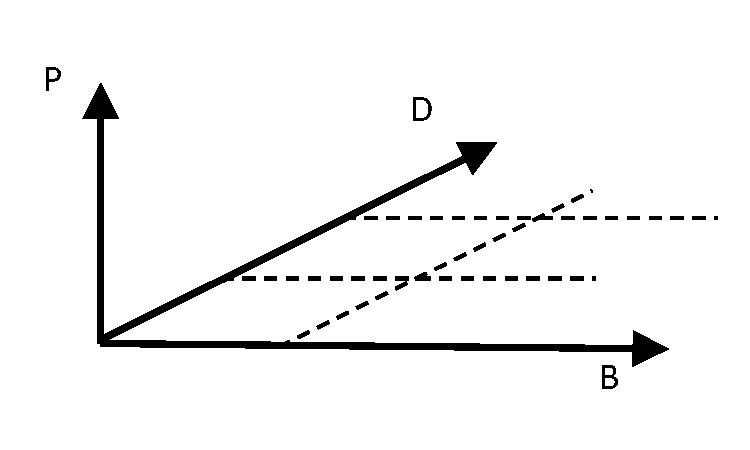
\includegraphics[width= 1.1\linewidth ]{figures/joint_axes}
  \end{center}
  \note[item]{Here's one example of what that table might look like.}
  \note[item]{What does the pmf look like?  if this is the B-D plane,
    the pmf is zero almost everywhere.}  \note[item]{I can mark a set
    of points, which are the outcome set, where there is a spike that
    comes out of the plane.  For example, there is some probability
    that the customer buys after 2 test drives.}  \note[item]{This
    type of graph is not very helpful to use, I just want you to get
    the picture in your mind}
\end{frame}

\begin{frame}
  \frametitle{The Joint Cumulative Probability Function}
  $$F(b,d) = P(B \leq b, D \leq d)$$
  
  \begin{itemize}
  \item Recall that $F_{X}(x) = \int_{-\infty}^{x}f(x)$ relates the CDF
    and PDF for the single variable case.
  \item In a similar way:
    $$F_{Y,X} = \int_{-\infty}^{x}\int_{-\infty}^{y}f(y,x) dy dx$$
  \item This can be hard to work with but can describe \textit{any}
    random variables.
  \end{itemize}
  
  \note[item]{Just like for one random variable, we can define a
    cumulative probability function for 2 or more random variables.}
  \note[item]{For almost everything, this is an inconvenient way to
    work with random variables} \note[item]{There is one giant
    advantage - this works to describe any random variables, discrete,
    continuous, or mixed.}  \note[item]{So probability theorists want
    to prove things using CDFs because that makes the results
    universal.}
\end{frame}

\subsection{Learnosity: The Probability Mass Function}

\begin{frame}
  \frametitle{Learnosity: The Probability Mass Function}
  
  Suppose that $X_1$ is a Bernoulli random variable representing a
  fair coin.  Suppose that $X_2$ is a Bernoulli random variable
  representing a second fair coin.  Let $Y = X_1 + X_2$.
  
  Fill in the following table for the PMF of $X_1$ and $Y$.
  
  \begin{tabular}{c|c|c}
    & $X_1 = 0$ & $X_1 = 1$ \\
    $Y=0$ & &  \\  
    $Y=1$ &  & \\  
    $Y=2$ & & \\
  \end{tabular}
\end{frame}

\subsection{Discrete Marginal and Conditional Distributions} 

\subsection{Reading Assignment: Discrete Marginal and Conditional
  Distributions}

\begin{frame}
  \frametitle{Reading Assignment}
  Read \textit{Foundations of Agnostic Statistics}, section 1.3.2.
\end{frame}

\subsection{Discrete Marginal Distributions}


\begin{frame}
  \frametitle{Marginal vs. Joint Distributions}
  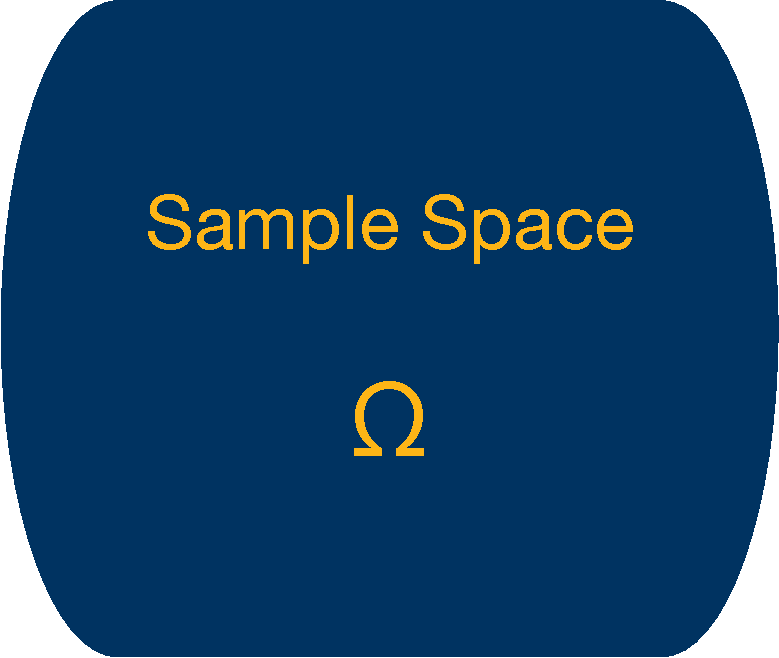
\includegraphics[width= .4\textwidth ]{figures/sample_space}

  \note[]{  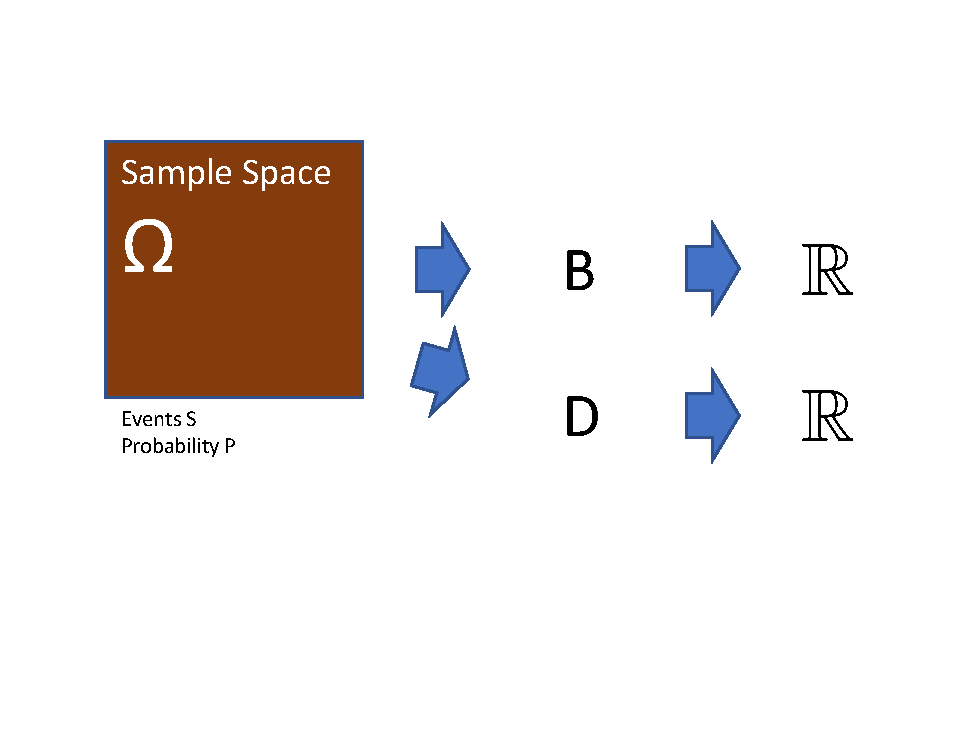
\includegraphics[width= \textwidth
    ]{figures/two_random_vars}} 
  \note[item]{Let's go back again to our car dealer example}
  \note[item]{You've created a customer model with two random
    variables: B for the Buy decision and D for number of cars taken
    for a test drive.}  \note[item]{If you think about it, you already
    have three ways to view this model} \note[item]{These are discrete
    random variables, so you can fully describe their joint
    distribution with a joint pmf} \note[item]{But also, you may want
    to look at each one individually} \note[item]{Suppose that the
    inventory department comes to you and says they need to understand
    just the buy decision, B} \note[item]{Well, there's no reason you
    can't study B by itself.  We know from earlier that we can
    describe B with a one dimensional probability mass function}
  \note[item]{In this context, we would call that B's marginal
    distribution.}  \note[item]{So we have three pmf's, and it's
    important to understand how they are related to each other.}
\end{frame}

\begin{frame}
  \frametitle{From Joint to Marginal Distributions}
 
  \note[item]{The book has this theorem that tell us how to go from a
    joint distribution to a marginal distribution}
  $$f_B(b) = P(B=b) = \sum_{d \in \text{Supp}[D]} f(b,d) \text{ for all } b \in \R$$
  
  \begin{tabular}[t]{c | c | c}
    & $B = 0$ & $B = 1$ \\
    \hline
    $D=0$ & .1   & .1  \\  
    $D=1$ &  .4  &  .1 \\  
    $D=2$ &  .1  &  .2 \\
  \end{tabular} 

  \note[item]{The first thing to notice is that to get the marginal
    distribution of B, we take a sum over all values of D}
  \note[item]{Let's see how that works in this table.  We want the
    probability that the customer buys a car, $f_B(1)$.}
  \note[item]{What do we do?  we have to sum up all the table cells
    that correspond to $B=1$... }  \note[item]{I'll write the sum down
    here - in the margin (that's why this is called the marginal
    distribution!)}  \note[item]{similarly, we can find the
    probability that the customer doesn't buy, $f_B(0)$, we just sum
    the other columm.}
\end{frame}

\begin{frame}
  \frametitle{From Marginal to Joint Distributions?}
  
  Is it possible to compute the joint distribution, $f$, given the
  marginals $f_B$ and $f_D$?  \note[item]{Let me do the first, then
    take 30 seconds to think about it, then click play again.  (unless
    it's worth turning into a learnosity quiz? but really just a brain
    teaser, we haven't taught students how to think about this.}

  \begin{center}
    \begin{tabular}[t]{c | c | c |c}
      & $B = 0$ & $B = 1$  & $F_D$ \\
      \hline
      $D=0$ &    &  & 0.2  \\  
      $D=1$ &    &   & 0.5 \\
      $D=2$ &   &   & 0.3  \\
      \hline
      $F_B$    & 0.6 & 0.4  &     
    \end{tabular}
  \end{center}

  \note[item]{the answer is no.  there is much more information in the
    joint distribution.}  \note[item]{In statistics, we have what are
    called degrees of freedom, which are like the dimensions along
    which the numbers can change.  If you look at $F_B$ there are two
    numbers, but you have one degree of freedom, because once you
    choose one of these probabilities, the other is determined.  For
    $F_D$ you have 2 degrees of freedom.  But for the joint, you have
    5.  So there's just too much information there.}  \note[item]{If
    you need more convincing, here are two different joint
    distributions that have the same marginals.}
\end{frame}

\begin{frame}
  \frametitle{From Marginal to Joint Distributions? (cont.)}
  \note[item]{ \alex{What if we fill in the table while we talk about
      this, rather than providing it to the students filled out?}
    \paul{I'm game, moving the filled version to notes}}
    Two joint distributions with the same marginals:
    
    \vspace{1cm}
  \begin{tabular}{c c}
    \begin{tabular}[t]{c | c | c |c}
      & $B = 0$ & $B = 1$  & $F_D$ \\
      \hline
      $D=0$ & 0.1   & 0.1  & 0.2  \\  
      $D=1$ & 0.4   & 0.1  & 0.5 \\
      $D=2$ & 0.1  & 0.2  & 0.3  \\
      \hline
      $F_B$    & 0.6 & 0.4  & \\
    \end{tabular} 
      &
        \begin{tabular}[t]{c | c | c |c}
          & $B = 0$ & $B = 1$  & $F_D$ \\
          \hline
          $D=0$ &   &  & 0.2  \\  
          $D=1$ &  &  & 0.5 \\
          $D=2$ &  &  & 0.3  \\
          \hline
          $F_B$    & 0.6 & 0.4  & \\
        \end{tabular}  
    \note[item]{
    \begin{tabular}[t]{c | c | c |c}
      & $B = 0$ & $B = 1$  & $F_D$ \\
      \hline
      $D=0$ & .2   & .0  & .2  \\  
      $D=1$ & .2   & .3  & .5 \\
      $D=2$ & .2  & .1  & .3  \\
      \hline
      $F_B$    & .6 & .4  & \\
    \end{tabular}  
    }
  \end{tabular}
\end{frame}

\subsection{Discrete Conditional Distributions}

\begin{frame}
  \frametitle{The Conditional PMF}

  \begin{itemize}
  \item Given two test drives ($D = 2$), what does the model say about
    buying behavior ($B$)?
  \item What is the conditional pmf, $f_{B|D}$?
  \end{itemize}

  \begin{center}
    \begin{tabular}[t]{c | c | c |c}
      & $B = 0$ & $B = 1$  & $F_D$ \\
      \hline
      $D=0$ & 0.1   & 0.1  & 0.2  \\  
      $D=1$ & 0.4   & 0.1  & 0.5 \\
      $D=2$ & 0.1  & 0.2  & 0.3  \\
      \hline
      $F_B$    & 0.6 & 0.4  & \\
    \end{tabular}
  \end{center}
  
  \note[item]{Let's go back again to the car dealer example.  You have
    modeled the joint distribution of the Buy decision B and the
    number of test drives D.}  \note[item]{Now a dealer comes to you
    and says that they have a customer that test drove 2 cars.  They
    want to know, according to your model, what probabilities to
    assign to buy and not buy.}  \note[item]{Since we know $D=2$, we
    can circle this row of the table.  we know we're here, so we can
    ignore the other numbers.  you can see that buying has twice the
    probability of not buying.}  \note[item]{but there's a problem.
    this is not a probability distribution, because the sum is not 1.}
  \note[item]{So, the solution is that we remember that probabilities
    are ratios, so we have to divide these by their total.  by the
    way, their total is exactly the marginal probability here - 0.3.
    when we divide then, we get 1/3 and 2/3.}
\end{frame}

\begin{frame}
  \frametitle{The Conditional PMF (cont.)}
  \note[item]{Here's the theorem from the book} \note[item]{We want
    the conditional distribution at some point b, given little d.
    This is a conditional probability, that B=b, given D = d.  we use
    the definition of conditional prob to write this as a fraction.
    then notice that we have the joint distribution over the
    marginal.}
  \begin{block}{Conditional expectation, car dealers}
    \begin{align*}
      f_{B|D}(b|d) & = P(B=b | D=d) \\
                   &= \frac{P(B=b, D=d)}{P(D=d)} = \frac{f(b,d)}{f_D(d)}
    \end{align*}
  \end{block}
  \pause \vspace{.5cm}
  $$
  \text{conditional} = \frac{\text{joint}}{\text{marginal}} \Leftrightarrow
  \pause \text{joint} = \text{marginal} \cdot
  \text{conditional}
  $$ 
  \note[item]{These are really just distributional versions of the
    multiplication rule we saw for events}
\end{frame}


\subsection{Reading: Jointly Continuous Random Variables}

\begin{frame}
  \frametitle{Reading Assignment}
  Read \textit{Foundations of Agnostic Statistics}, section 1.3.3.
\end{frame}

\subsection{Jointly Continuous Random Variables}

\begin{frame}
  \frametitle{The Joint Density Function}
  \note[item]{Let's take a look at joint distributions for continuous
    random variables} \note[item]{Before we saw that when random
    variables are discrete, we can describe them with a joint pmf.
    now we need a joint density function} \note[item]{When you imagine
    a joint density, think about a surface.}  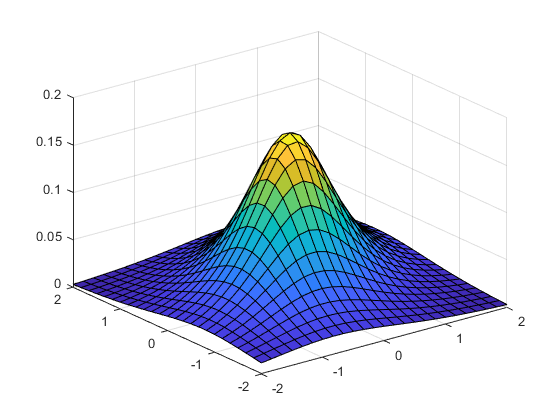
\includegraphics[width=
  \textwidth ]{figures/surface} \note[item]{The higher the surface in
    an area, the more probability you have there}
 
  \note[item]{Working with densities is a little less intuitive, but
    luckily, most of what we have to do is remember what we did for
    discrete random variables, and turn the sums into integral}
\end{frame}


\begin{frame}
  \frametitle{Probabilities of Events}
  
  \hskip-1cm
  \begin{tabular}{p{0.7\textwidth} p{0.3\textwidth}}
    \vspace{0pt} 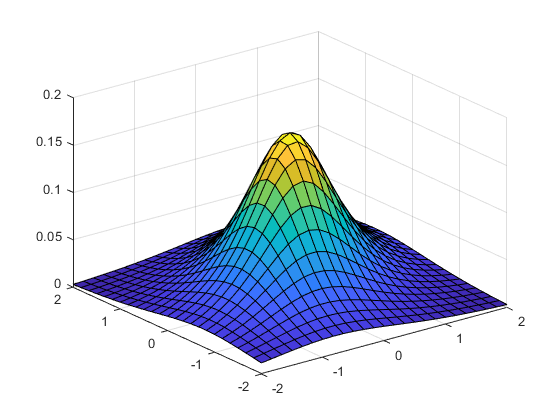
\includegraphics[width= \linewidth ]{figures/surface}
    & \vspace{15pt} How to compute: $P((X,Y) \in A)$
  \end{tabular}
  \note[item]{The first thing we might want to do is
    compute the probability that (X,Y) is in some set. -
    Let's draw some set D on the X-Y plane}
  \note[item]{When we had discrete random variables, we
    summed up the pmf for all points in that set.}
  \note[item]{Now we have to take an integral over that
    area}
  \note[item]{$P((X,Y) \in D) = \int \int_{(x,y) \in D}
    f(x,y) dx dy$}
\end{frame}

\begin{frame}
  \frametitle{Continuous Marginal Distributions}
  \hskip-1cm
  \begin{tabular}{p{0.7\textwidth} p{0.3\textwidth}}
    \vspace{0pt} 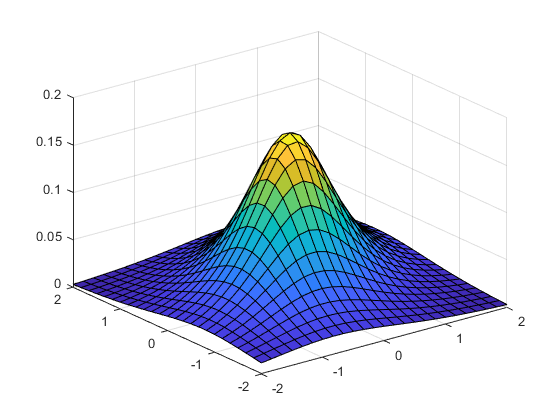
\includegraphics[width= \linewidth ]{figures/surface}
    & \vspace{15pt} How to compute: $f_X(x)$
  \end{tabular}
  \note[item]{Next, how do we compute a marginal
    distribution?}  \note[item]{Let's choose a specific X,
    $X=x$.  When we had discrete random variables, we would
    take a sum across the row for that x.}  \note[item]{Now
    that X defines a slice through this surface}
  \note[item]{Instead of a sum, now we take an integral of
    that slice..}  \note[item]{That will give us the value
    of the marginal density of X at that x.}
  \note[item]{$f_X(x) = \int_{-\infty}^\infty f(x,y) dy$}
\end{frame}

\begin{frame}
  \frametitle{Continuous Conditional Distributions}
  \hskip-1cm
  \begin{tabular}{p{0.7\textwidth}
    p{0.3\textwidth}} \vspace{0pt}
    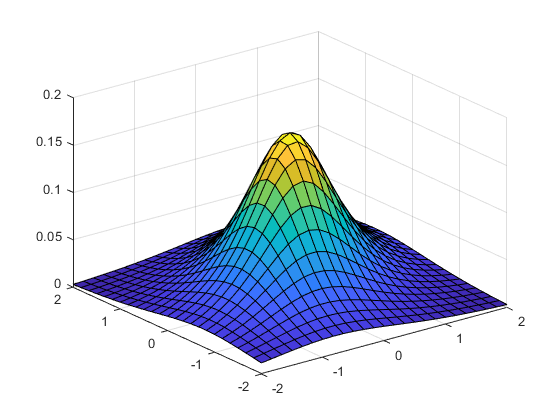
\includegraphics[width= \linewidth ]{figures/surface} &
                                                            \vspace{15pt} How to compute: $f_{B|D}(b|d) $ \pause
 \end{tabular}
  $$\text{conditional} = \frac{\text{joint}}{\text{marginal}}$$
  
  \note[item]{Finally, how do we compute a conditional distribution?}
  \note[item]{Let's choose a specific X, $X=x$.  When we condition on
    that x, it's like we're saying that we know we're somewhere in that
    slice.}  \note[item]{So the shape of the slice tells us exactly how
    probable one value of y is compared to another} \note[item]{But just
    like for discrete random variables, we have to scale things to make
    sure the total probability is 1.}
  \note[item]{$$f_{B|D}(b|d) = \frac{f(b,d)}{f_D(d)}$$} \note[item]{So
    this equation is exactly the same as before! but now these are
    densities instead of probability masses.}
\end{frame}

\subsection{Reading: Independent Random Variables} 

\begin{frame}
  \frametitle{Reading Assignment}
  Read \textit{Foundations of Agnostic Statistics}, section 1.3.4.
\end{frame}

\subsection{Independent Random Variables}

\begin{frame}
  \frametitle{Independence}
  \note[item]{Independence is a key property that we will use again
    and again in this course} \note[item]{First, let's look at the
    definition...}  If $X$ and $Y$ are independent, $X \indep Y$.
  
  \begin{enumerate}
    \pause
  \item The marginals fully describe the distribution:
    
    $f(x,y) = f_X(x)f_Y(y)$ \pause
  \item Knowing X tells you nothing about Y:
    
    $f_{Y|X}(y|x) =$ \note[item]{
      $ \frac{f(x,y)}{f_X(x)} = \frac{f_X(x)f_Y(y)}{f_X(x)} = f_Y(y)$ }
  \end{enumerate}
\end{frame}

\begin{frame}
  \frametitle{Drawing Independent Continuous RV}

  \note[item]{Draw a normal curve in two dimensions, but linear in
    one.}
  \note[]{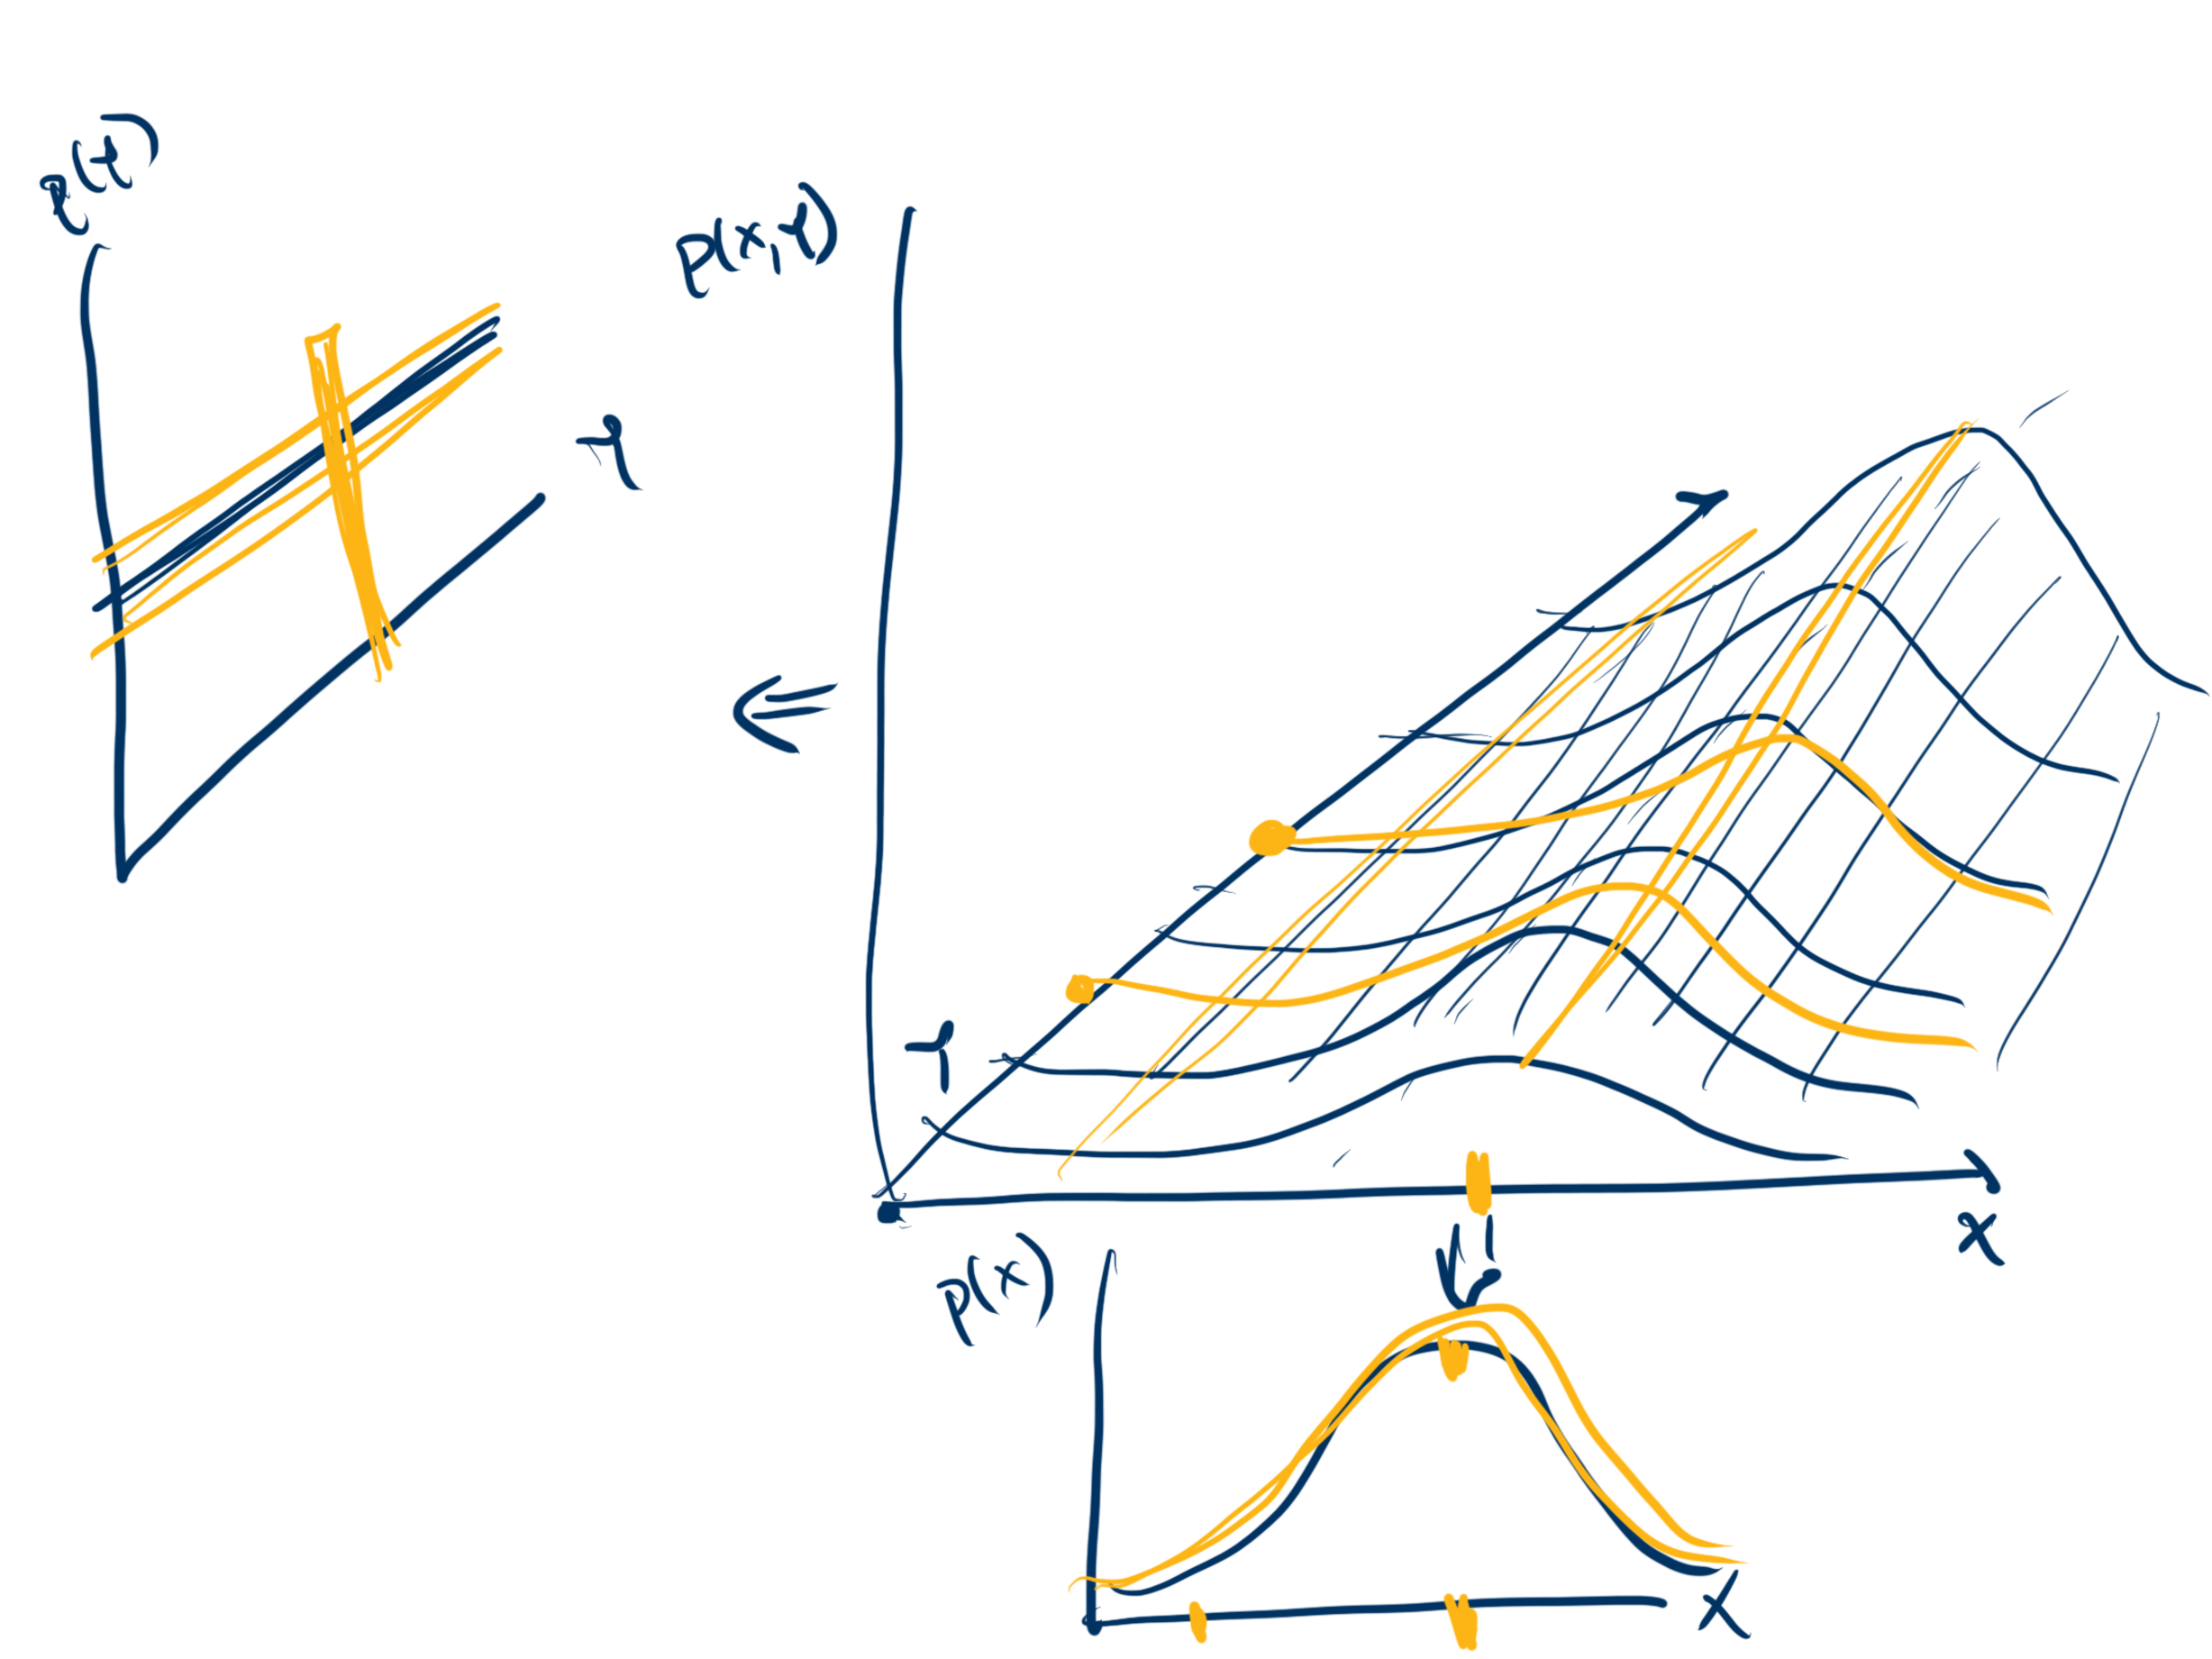
\includegraphics[width=.7\linewidth]{figures/independent_rv}}
\end{frame}

\begin{frame}
  \frametitle{Drawing Non-Independent Continuous RV}

  \note[item]{Draw a normal curve in two dimensions}
  \note[item]{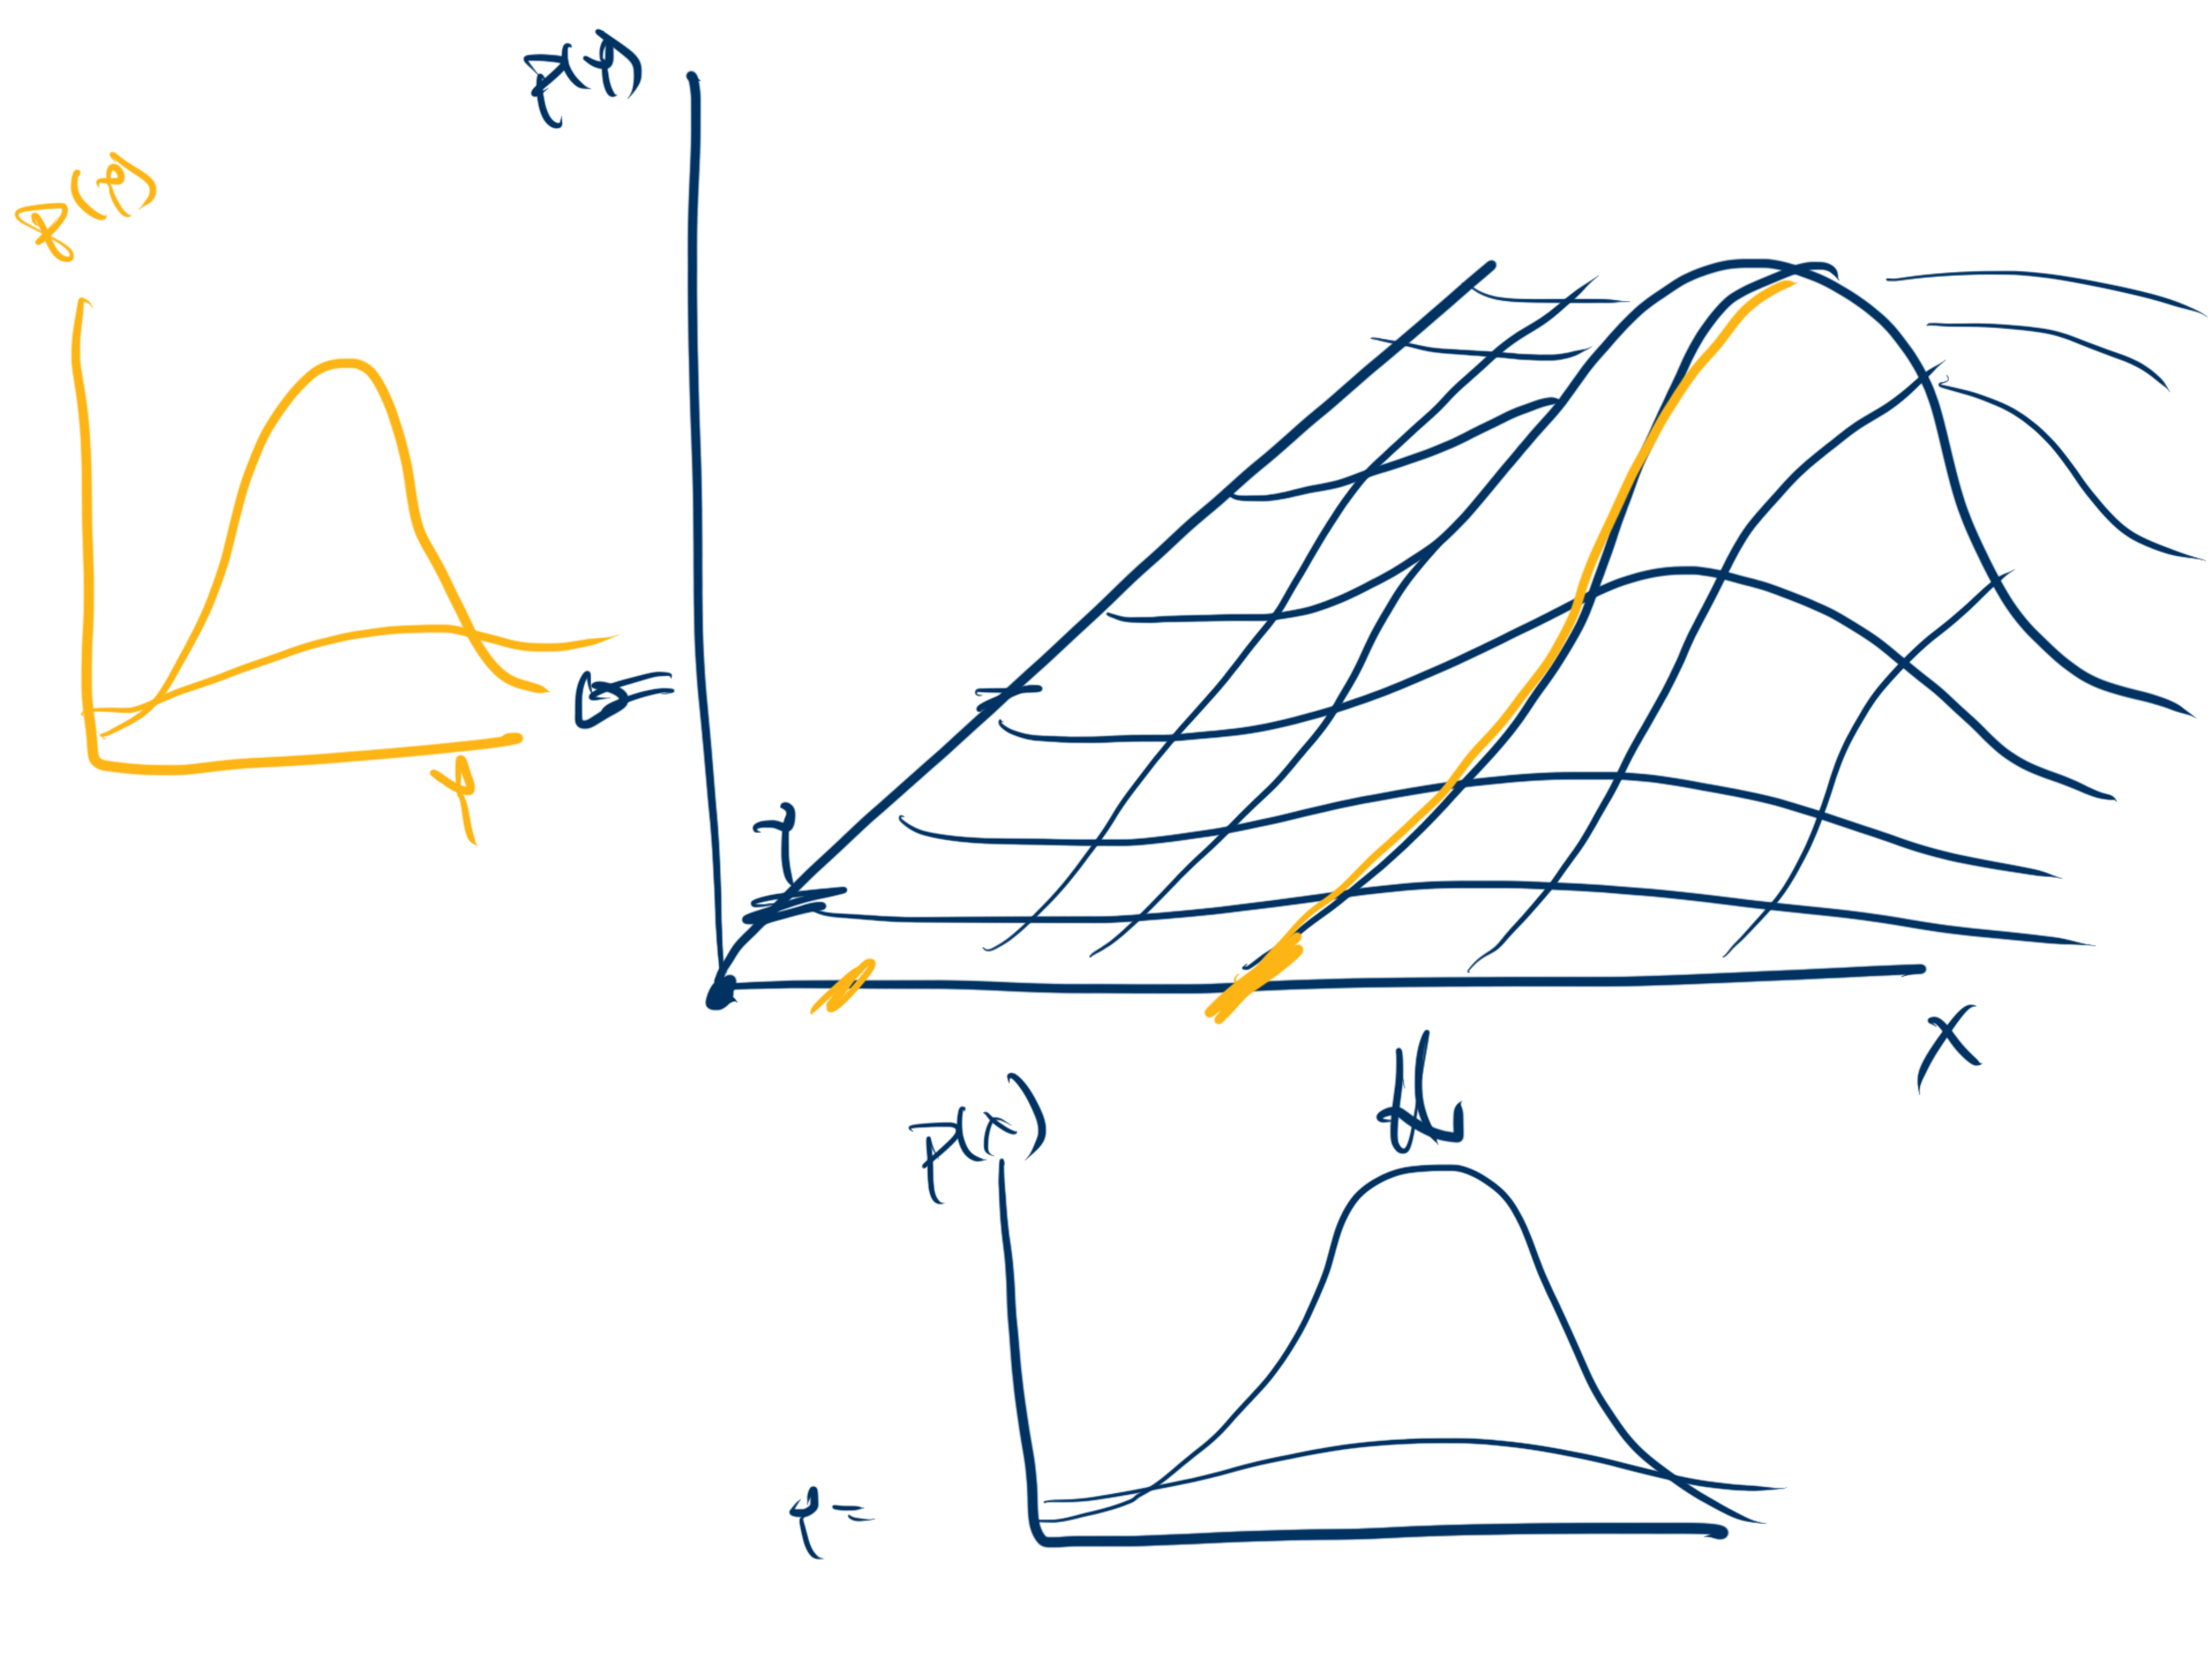
\includegraphics[width=.7\linewidth]{figures/non-independent_rv}}
\end{frame} 


\begin{frame}
  \frametitle{Importance of Independence}
  \note[item]{The reason independence is so important will come when
    we try to fit our models to data} $B_1$ represents blood pressure
  of patient 1.

  $B_2$ represents blood pressure of patient 2.

  \vdots

  Without simplifying assumptions, the joint distribution of
  $B_1, B_2,...$ is too complex to estimate with limited data.

  Independence $\implies$ only need to estimate the marginals

  \note[item]{we'll see how this process works when we get to
    estimators.}

\end{frame}


\begin{frame}
  \frametitle{Assessing Independence in Practice}
  
  Independence is rarely (if ever) perfectly met.
  
  What if:
  \begin{itemize}
  \item Patient 1 and patient 2 are related
  \item Technicians trade off every 10 patients
  \item After seeing an unusually high blood pressure, the technician
    adjusts their mannerisms
  \end{itemize}
  
  These are potential \textit{dependencies}.  \note[item]{Remember,
    there will almost always be some.  It's important to identify
    them.  But you must exercise judgement about which are really
    important and which are minor.}  \note[item]{\paul{Maybe delete
      this slide since you probably cover all this in week 4.}}
\end{frame}




\end{document}
